\documentclass[]{book}
\usepackage{lmodern}
\usepackage{amssymb,amsmath}
\usepackage{ifxetex,ifluatex}
\usepackage{fixltx2e} % provides \textsubscript
\ifnum 0\ifxetex 1\fi\ifluatex 1\fi=0 % if pdftex
  \usepackage[T1]{fontenc}
  \usepackage[utf8]{inputenc}
\else % if luatex or xelatex
  \ifxetex
    \usepackage{mathspec}
  \else
    \usepackage{fontspec}
  \fi
  \defaultfontfeatures{Ligatures=TeX,Scale=MatchLowercase}
\fi
% use upquote if available, for straight quotes in verbatim environments
\IfFileExists{upquote.sty}{\usepackage{upquote}}{}
% use microtype if available
\IfFileExists{microtype.sty}{%
\usepackage{microtype}
\UseMicrotypeSet[protrusion]{basicmath} % disable protrusion for tt fonts
}{}
\usepackage[margin=1in]{geometry}
\usepackage{hyperref}
\hypersetup{unicode=true,
            pdftitle={Supplement to Shiny in Production},
            pdfborder={0 0 0},
            breaklinks=true}
\urlstyle{same}  % don't use monospace font for urls
\usepackage{natbib}
\bibliographystyle{plainnat}
\usepackage{color}
\usepackage{fancyvrb}
\newcommand{\VerbBar}{|}
\newcommand{\VERB}{\Verb[commandchars=\\\{\}]}
\DefineVerbatimEnvironment{Highlighting}{Verbatim}{commandchars=\\\{\}}
% Add ',fontsize=\small' for more characters per line
\usepackage{framed}
\definecolor{shadecolor}{RGB}{248,248,248}
\newenvironment{Shaded}{\begin{snugshade}}{\end{snugshade}}
\newcommand{\AlertTok}[1]{\textcolor[rgb]{0.94,0.16,0.16}{#1}}
\newcommand{\AnnotationTok}[1]{\textcolor[rgb]{0.56,0.35,0.01}{\textbf{\textit{#1}}}}
\newcommand{\AttributeTok}[1]{\textcolor[rgb]{0.77,0.63,0.00}{#1}}
\newcommand{\BaseNTok}[1]{\textcolor[rgb]{0.00,0.00,0.81}{#1}}
\newcommand{\BuiltInTok}[1]{#1}
\newcommand{\CharTok}[1]{\textcolor[rgb]{0.31,0.60,0.02}{#1}}
\newcommand{\CommentTok}[1]{\textcolor[rgb]{0.56,0.35,0.01}{\textit{#1}}}
\newcommand{\CommentVarTok}[1]{\textcolor[rgb]{0.56,0.35,0.01}{\textbf{\textit{#1}}}}
\newcommand{\ConstantTok}[1]{\textcolor[rgb]{0.00,0.00,0.00}{#1}}
\newcommand{\ControlFlowTok}[1]{\textcolor[rgb]{0.13,0.29,0.53}{\textbf{#1}}}
\newcommand{\DataTypeTok}[1]{\textcolor[rgb]{0.13,0.29,0.53}{#1}}
\newcommand{\DecValTok}[1]{\textcolor[rgb]{0.00,0.00,0.81}{#1}}
\newcommand{\DocumentationTok}[1]{\textcolor[rgb]{0.56,0.35,0.01}{\textbf{\textit{#1}}}}
\newcommand{\ErrorTok}[1]{\textcolor[rgb]{0.64,0.00,0.00}{\textbf{#1}}}
\newcommand{\ExtensionTok}[1]{#1}
\newcommand{\FloatTok}[1]{\textcolor[rgb]{0.00,0.00,0.81}{#1}}
\newcommand{\FunctionTok}[1]{\textcolor[rgb]{0.00,0.00,0.00}{#1}}
\newcommand{\ImportTok}[1]{#1}
\newcommand{\InformationTok}[1]{\textcolor[rgb]{0.56,0.35,0.01}{\textbf{\textit{#1}}}}
\newcommand{\KeywordTok}[1]{\textcolor[rgb]{0.13,0.29,0.53}{\textbf{#1}}}
\newcommand{\NormalTok}[1]{#1}
\newcommand{\OperatorTok}[1]{\textcolor[rgb]{0.81,0.36,0.00}{\textbf{#1}}}
\newcommand{\OtherTok}[1]{\textcolor[rgb]{0.56,0.35,0.01}{#1}}
\newcommand{\PreprocessorTok}[1]{\textcolor[rgb]{0.56,0.35,0.01}{\textit{#1}}}
\newcommand{\RegionMarkerTok}[1]{#1}
\newcommand{\SpecialCharTok}[1]{\textcolor[rgb]{0.00,0.00,0.00}{#1}}
\newcommand{\SpecialStringTok}[1]{\textcolor[rgb]{0.31,0.60,0.02}{#1}}
\newcommand{\StringTok}[1]{\textcolor[rgb]{0.31,0.60,0.02}{#1}}
\newcommand{\VariableTok}[1]{\textcolor[rgb]{0.00,0.00,0.00}{#1}}
\newcommand{\VerbatimStringTok}[1]{\textcolor[rgb]{0.31,0.60,0.02}{#1}}
\newcommand{\WarningTok}[1]{\textcolor[rgb]{0.56,0.35,0.01}{\textbf{\textit{#1}}}}
\usepackage{longtable,booktabs}
\usepackage{graphicx,grffile}
\makeatletter
\def\maxwidth{\ifdim\Gin@nat@width>\linewidth\linewidth\else\Gin@nat@width\fi}
\def\maxheight{\ifdim\Gin@nat@height>\textheight\textheight\else\Gin@nat@height\fi}
\makeatother
% Scale images if necessary, so that they will not overflow the page
% margins by default, and it is still possible to overwrite the defaults
% using explicit options in \includegraphics[width, height, ...]{}
\setkeys{Gin}{width=\maxwidth,height=\maxheight,keepaspectratio}
\IfFileExists{parskip.sty}{%
\usepackage{parskip}
}{% else
\setlength{\parindent}{0pt}
\setlength{\parskip}{6pt plus 2pt minus 1pt}
}
\setlength{\emergencystretch}{3em}  % prevent overfull lines
\providecommand{\tightlist}{%
  \setlength{\itemsep}{0pt}\setlength{\parskip}{0pt}}
\setcounter{secnumdepth}{5}
% Redefines (sub)paragraphs to behave more like sections
\ifx\paragraph\undefined\else
\let\oldparagraph\paragraph
\renewcommand{\paragraph}[1]{\oldparagraph{#1}\mbox{}}
\fi
\ifx\subparagraph\undefined\else
\let\oldsubparagraph\subparagraph
\renewcommand{\subparagraph}[1]{\oldsubparagraph{#1}\mbox{}}
\fi

%%% Use protect on footnotes to avoid problems with footnotes in titles
\let\rmarkdownfootnote\footnote%
\def\footnote{\protect\rmarkdownfootnote}

%%% Change title format to be more compact
\usepackage{titling}

% Create subtitle command for use in maketitle
\newcommand{\subtitle}[1]{
  \posttitle{
    \begin{center}\large#1\end{center}
    }
}

\setlength{\droptitle}{-2em}

  \title{Supplement to Shiny in Production}
    \pretitle{\vspace{\droptitle}\centering\huge}
  \posttitle{\par}
    \author{}
    \preauthor{}\postauthor{}
      \predate{\centering\large\emph}
  \postdate{\par}
    \date{2019-01-13}

\usepackage{booktabs}

\usepackage{amsthm}
\newtheorem{theorem}{Theorem}[chapter]
\newtheorem{lemma}{Lemma}[chapter]
\theoremstyle{definition}
\newtheorem{definition}{Definition}[chapter]
\newtheorem{corollary}{Corollary}[chapter]
\newtheorem{proposition}{Proposition}[chapter]
\theoremstyle{definition}
\newtheorem{example}{Example}[chapter]
\theoremstyle{definition}
\newtheorem{exercise}{Exercise}[chapter]
\theoremstyle{remark}
\newtheorem*{remark}{Remark}
\newtheorem*{solution}{Solution}
\begin{document}
\maketitle

{
\setcounter{tocdepth}{1}
\tableofcontents
}
\hypertarget{shiny-in-production-workshop-rstudio-conf-2019}{%
\chapter{Shiny in Production Workshop @ RStudio Conf
2019}\label{shiny-in-production-workshop-rstudio-conf-2019}}

This document is full of supplemental resources and content from the
Shiny in Production Workshop delievered at rstudio::conf 2019.

The \textbf{bookdown} package can be installed from CRAN or Github:

\begin{Shaded}
\begin{Highlighting}[]
\KeywordTok{install.packages}\NormalTok{(}\StringTok{"bookdown"}\NormalTok{)}
\CommentTok{# or the development version}
\CommentTok{# devtools::install_github("rstudio/bookdown")}
\end{Highlighting}
\end{Shaded}

\hypertarget{course-intro}{%
\chapter{Introduction to Shiny in Production}\label{course-intro}}

\textbf{Why are we here?}

\begin{quote}
Shiny applications are being deployed in high-value, customer-facing,
and/or enterprise-wide scenarios. Unfortunately, they are often being
done without the benefit of best practices. This workshop will help you
and/or your IT colleagues who support your data scientists learn how to
accelerate a successful Shiny application deployment in production
scenarios.
\end{quote}

Over the past year, software developers at RStudio have been working
hard to dispel rumors that Shiny ``isn't ready and can't run in
production''. They've built a bunch of cool new tools that are useful in
preparing applications for production and understanding how to configure
and scale them for optimized performance and user experience.

This workshop will cover all these new tools for shiny development as
well as the equally important logistical pieces of a production story:

\begin{itemize}
\tightlist
\item
  What does production infrastructure and tooling look like for Shiny
  apps?
\item
  How do we get Shiny apps from development into production?
\item
  How are Shiny apps maintained production?
\end{itemize}

\begin{quote}
When developers begin to think of infrastructure as part of their
application, stability and performance become normative. - Jeff Geerling
``Ansible for DevOps''
\end{quote}

\hypertarget{workshop-objectives}{%
\section{Workshop Objectives}\label{workshop-objectives}}

\textbf{Running Shiny in Production}

\begin{itemize}
\tightlist
\item
  Is Shiny ready for production?
\item
  What does it take to get there?
\item
  What do you need to know?
\item
  What tools are available?
\item
  How do you develop a workflow?
\end{itemize}

\textbf{Understand the importance of incremental changes and testing}

\begin{itemize}
\tightlist
\item
  Version control
\item
  Tests for package upgrades
\item
  Use of separate environments for staging and production
\item
  Incorporating automated testing into a development workflow:
  \texttt{shinytest}
\end{itemize}

\textbf{Data product tradeoffs}

\begin{itemize}
\tightlist
\item
  What are the advantages to using Shiny vs Plumber vs R Markdown
\item
  What is the difference between a stateless Plumber API and a Shiny
  Session?
\end{itemize}

\textbf{Development vs.~Production environment considerations}

\begin{itemize}
\tightlist
\item
  Defining a data model

  \begin{itemize}
  \tightlist
  \item
    Working with databases
  \end{itemize}
\item
  Tools for understanding application performance

  \begin{itemize}
  \tightlist
  \item
    \texttt{shinyloadtest}
  \item
    \texttt{profvis}
  \end{itemize}
\item
  Tools for improving application performance

  \begin{itemize}
  \tightlist
  \item
    Plot caching
  \item
    Synchronous vs asynchronous paradigms: \texttt{async}
  \end{itemize}
\end{itemize}

\textbf{Deployment architecture and tools}

\begin{itemize}
\tightlist
\item
  Introduction to analytic infrastructure
\item
  Configuration management
\item
  Resources for scaling horizontally
\end{itemize}

\hypertarget{workshop-infrastructure}{%
\section{Workshop Infrastructure}\label{workshop-infrastructure}}

\begin{itemize}
\tightlist
\item
  RStudio Connect
\item
  PostgreSQL
\item
  RStudio Server Pro
\end{itemize}

Instructions for accessing the classroom environment are available in
the workshop slide deck.

\hypertarget{app-intro}{%
\chapter{Introduction to the Application}\label{app-intro}}

\textbf{Every Application has an Origin Story}

Data Scientists at RStudio University have discovered that there are
trackable traits and behaviors students engage in that have been
predictive of the desired 4-year graduation track.

They have built a shiny application that can be used by the very
data-savvy advisors at this illustrious institution to identify students
in need of guidance and show them the top behavioral factors driving
individual predictions coming out of the model.

\begin{figure}
\centering
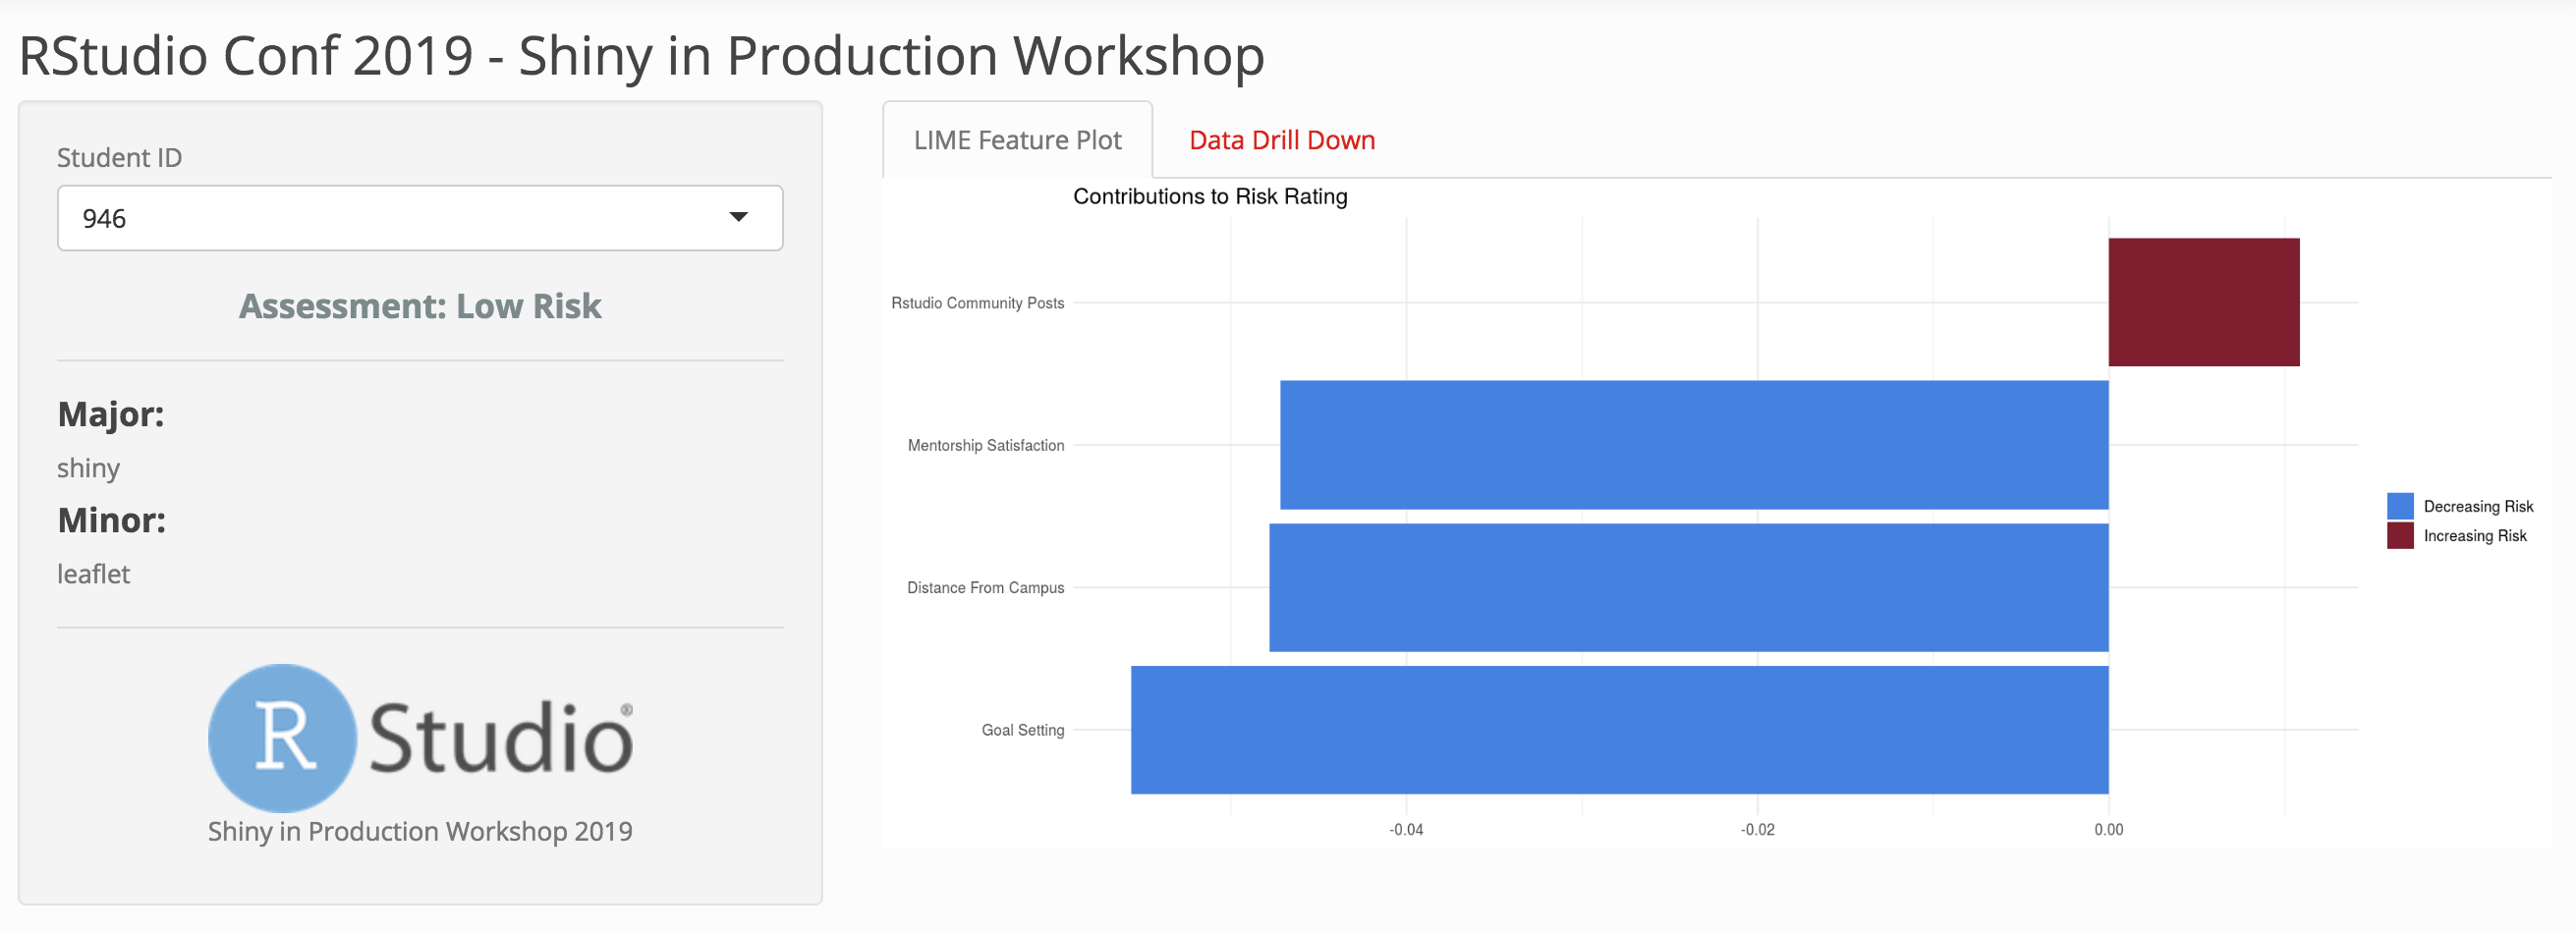
\includegraphics{imgs/app-intro/app-screenshot.png}
\caption{App Preview}
\end{figure}

The POC was a smashing success - but now \emph{our advisors actually
want to use this thing for real}.

\begin{itemize}
\tightlist
\item
  We've developed a nice app
\item
  We want to put it into production
\item
  We want confidence that it will perform well in production, both now
  and in the future
\end{itemize}

\hypertarget{activity-explore-the-application}{%
\section{Activity: Explore the
Application}\label{activity-explore-the-application}}

\emph{First: Open \texttt{app.R} and Run the Application}

\textbf{Discussion: Explore the Application}

\begin{itemize}
\tightlist
\item
  Are there any parts of the app code that don't make sense?
\item
  Is this application ready for production?
\item
  How would you define ``production''?
\item
  What insights would be useful to have about the application before we
  try to deploy it?
\end{itemize}

\emph{Additional Discussion:}

\begin{itemize}
\tightlist
\item
  What is your current process for taking applications into production?
\end{itemize}

\textbf{Deliverable: Start a Plan}

\begin{itemize}
\tightlist
\item
  Create a checklist
\item
  Outline the steps you might take to put this application into
  production
\end{itemize}

\textbf{Checklist for Taking Applications into Production}

A high-level Checklist to build off of:

\begin{figure}
\centering
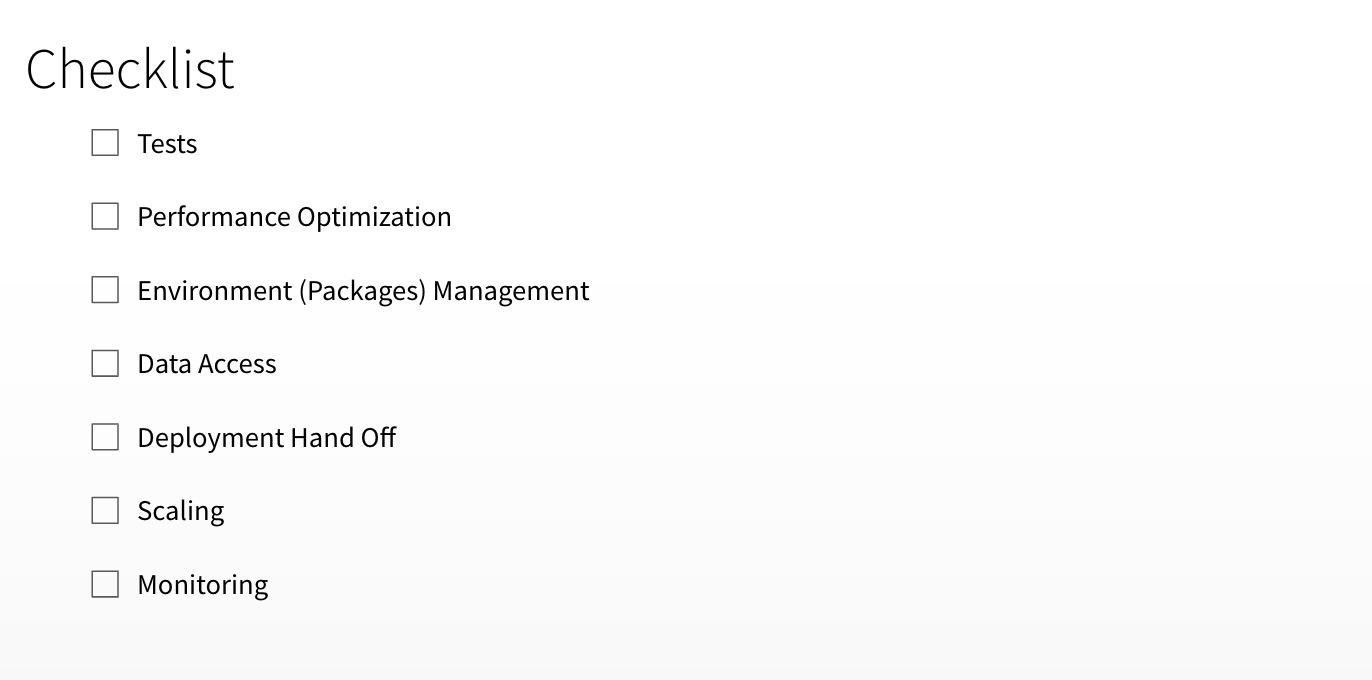
\includegraphics{imgs/app-intro/skeleton-checklist.png}
\caption{Ideas for Getting Started: Checklist}
\end{figure}

\hypertarget{application-testing-shinytest}{%
\chapter{\texorpdfstring{Application Testing:
\texttt{shinytest}}{Application Testing: shinytest}}\label{application-testing-shinytest}}

\begin{itemize}
\tightlist
\item
  You've developed a nice app
\item
  You've put it in production
\item
  You want to be confident that it will keep running in the future
\end{itemize}

\textbf{Things that can change/break a Shiny application}

\begin{itemize}
\tightlist
\item
  Modifying code
\item
  Upgrading the \texttt{shiny} package
\item
  Upgrading other packages
\item
  Upgrading R
\item
  External data source changes or fails
\end{itemize}

\hypertarget{testing-options}{%
\subsubsection{Testing Options}\label{testing-options}}

\begin{itemize}
\tightlist
\item
  Manual testing

  \begin{itemize}
  \tightlist
  \item
    time intensive
  \item
    inconsistent
  \end{itemize}
\item
  Automated testing (hard)

  \begin{itemize}
  \tightlist
  \item
    web browser
  \item
    simulated user interactions
  \item
    tests for graphical elements
  \end{itemize}
\end{itemize}

Enter: Snapshot-based testing
\href{https://github.com/rstudio/webinars/blob/master/48-shinytest/shinytest.pdf}{Webinar
Slide Deck}

\begin{figure}
\centering
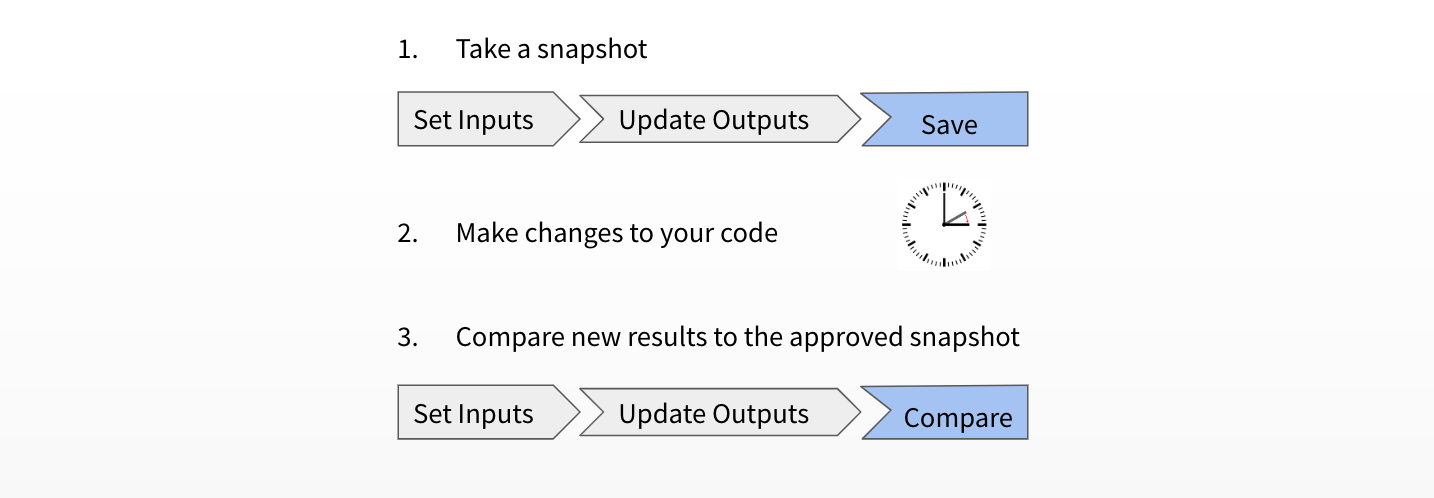
\includegraphics{imgs/testing/snapshot-testing.png}
\caption{Snapshot Testing}
\end{figure}

\begin{itemize}
\tightlist
\item
  Can be easier to create tests
\item
  Can test an entire application
\item
  More sensitive to spurious changes
\end{itemize}

\hypertarget{automated-testing-for-shiny-apps}{%
\subsubsection{Automated Testing for Shiny
Apps}\label{automated-testing-for-shiny-apps}}

\begin{itemize}
\tightlist
\item
  \href{https://resources.rstudio.com/rstudio-blog/shinytest-automated-testing-for-shiny-apps}{Blog}
\end{itemize}

\texttt{shinytest} is a package (available on CRAN) to perform automated
testing for Shiny apps.

Basic \texttt{shinytest} proceedure:

\begin{figure}
\centering
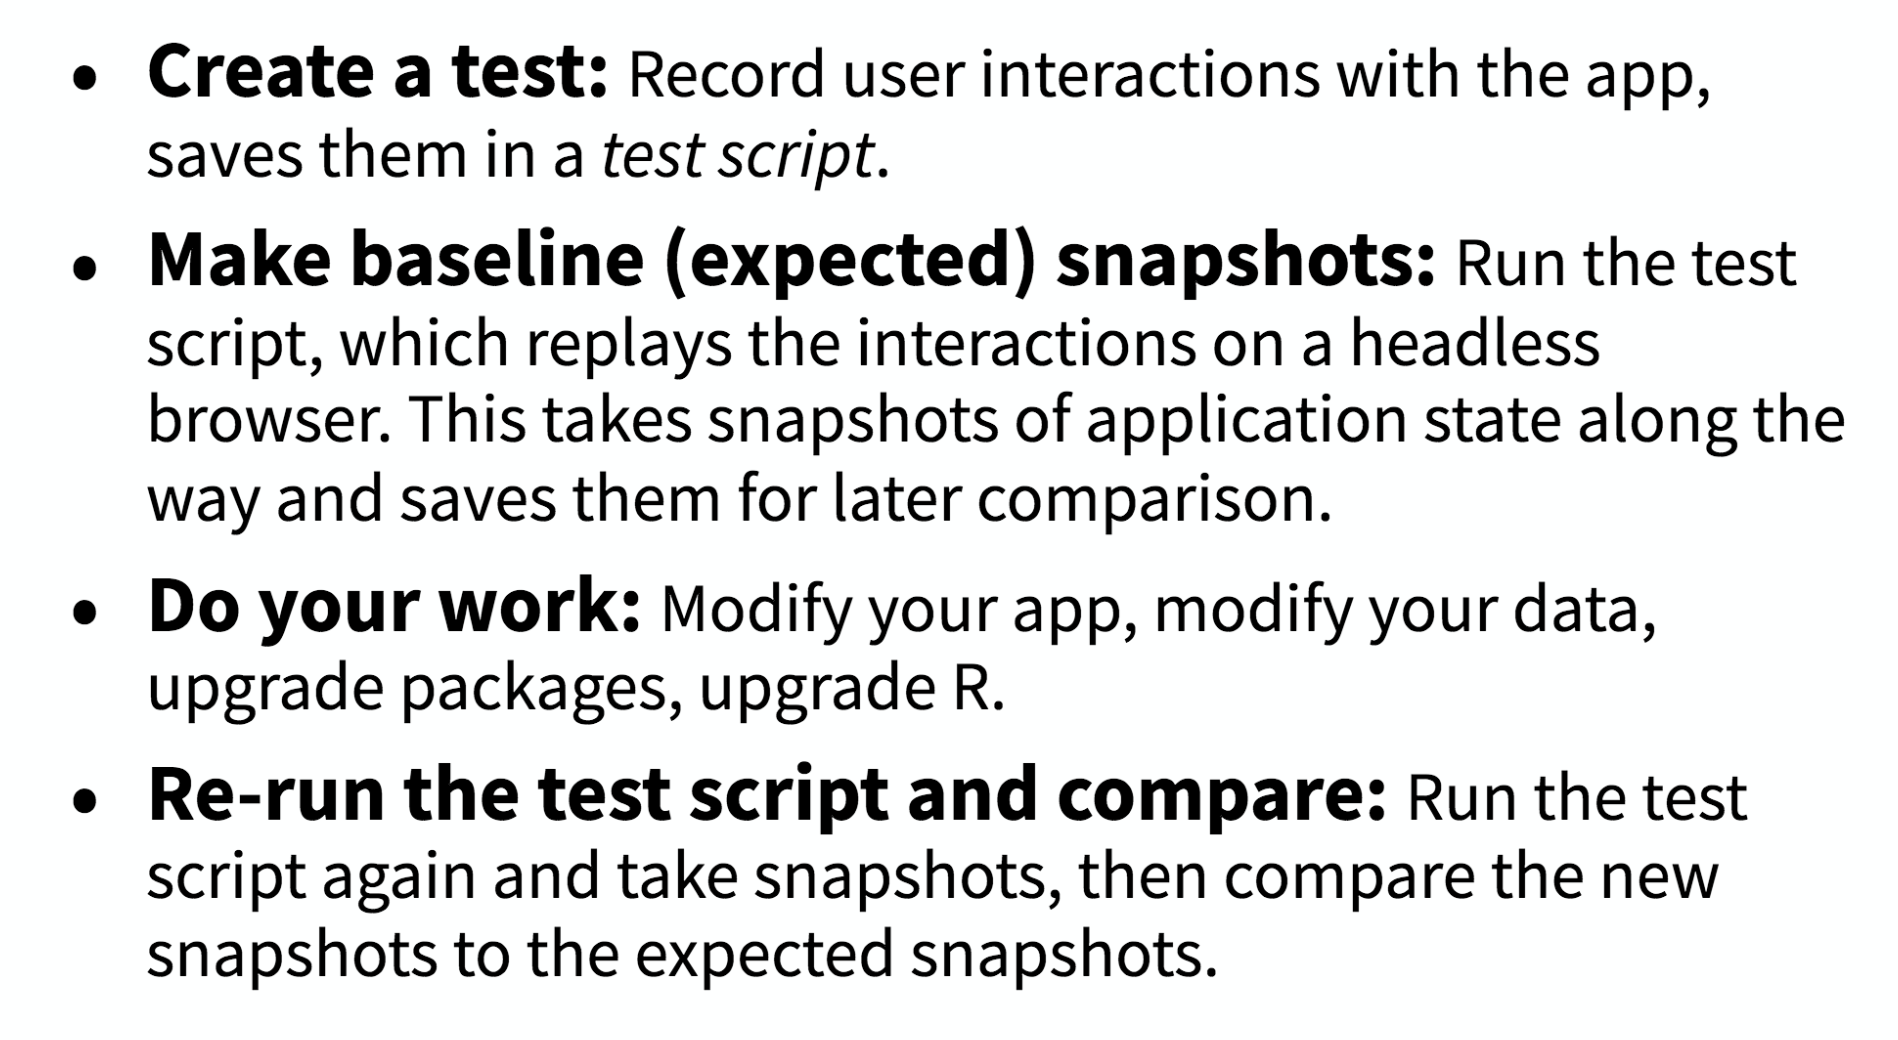
\includegraphics{imgs/testing/testing-proceedure.png}
\caption{shinytest proceedure}
\end{figure}

Support for \texttt{shinytest} is available in RStudio v1.2 preview.

\textbf{Installation}

`install.packages(``shinytest'')

\textbf{Note:} When running \texttt{shinytest} for the first time, you
may be prompted by the RStudio IDE or package warning messages to
install some dependencies. \texttt{shinytest} requires a headless web
browser (PhantomJS) to record and run tests.

\begin{itemize}
\tightlist
\item
  To install it, run shinytest::installDependencies()
\item
  If it is installed, make sure the phantomjs executable can be found
  via the PATH variable.
\end{itemize}

\textbf{Record Tests}

\begin{itemize}
\tightlist
\item
  Run \texttt{recordTest()} to launch the app in a test recorder.
\item
  Create the tests by interacting with the application - this will allow
  the recorder to snapshot the application state at various points.
\item
  Quit the test recorder. This action will trigger the following events:

  \begin{itemize}
  \tightlist
  \item
    The test script will be saved as a .R file in a subdirectory of the
    application named \texttt{tests/}.
  \item
    If you are running in the RStudio IDE, it will automatically open
    this file in the editor.
  \item
    The test script will be run, and the snapshots will be saved in a
    subdirectory of the \texttt{tests/} directory.
  \end{itemize}
\end{itemize}

To record tests from \texttt{R}, run the following:

\begin{verbatim}
library(shinytest)

recordTest("path/to/the/app")   #Replace with the correct path
\end{verbatim}

To record tests from RStudio v1.2, when an application file (app.R,
server.R, ui.R or global.R) is open in the editor, a button labeled
\emph{Run App} will appear at the top of the editor pane. Click on the
small black triangle next to this button to reveal the menu of extended
options.

\begin{figure}
\centering
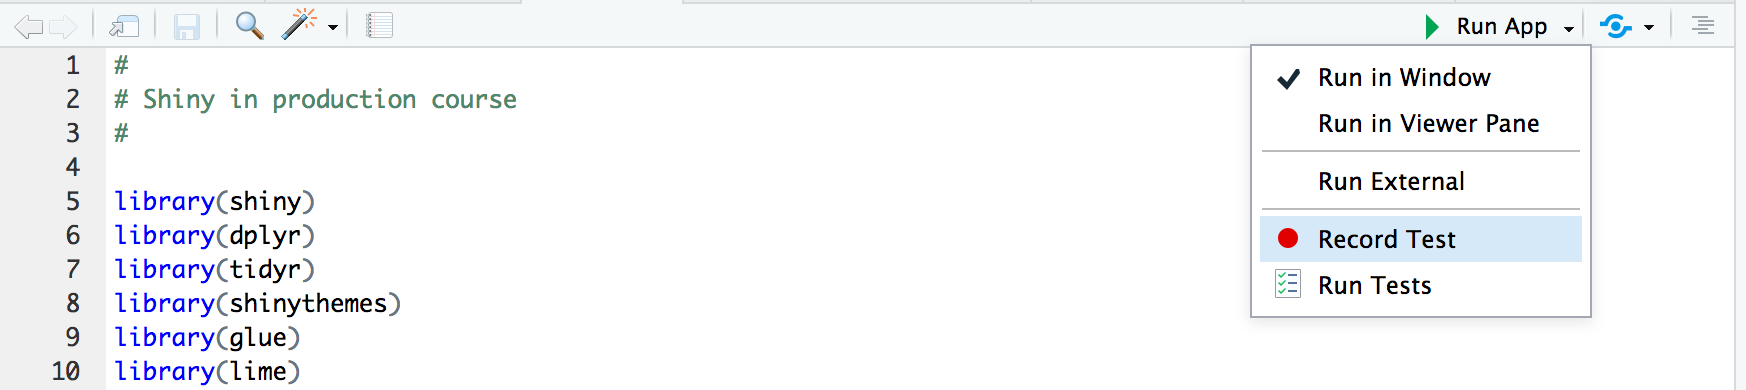
\includegraphics{imgs/testing/record_test_button.png}
\caption{Record Test Button}
\end{figure}

This launches the Shiny application to be tested in a separate R
process. We'll refer to this as the \textbf{target app}. At the same
time, the current R process lauches a special Shiny application which
displays the target app in an iframe along with some controls. We'll
refer to this as the \textbf{recorder app}. You should see something
like this:

\begin{figure}
\centering
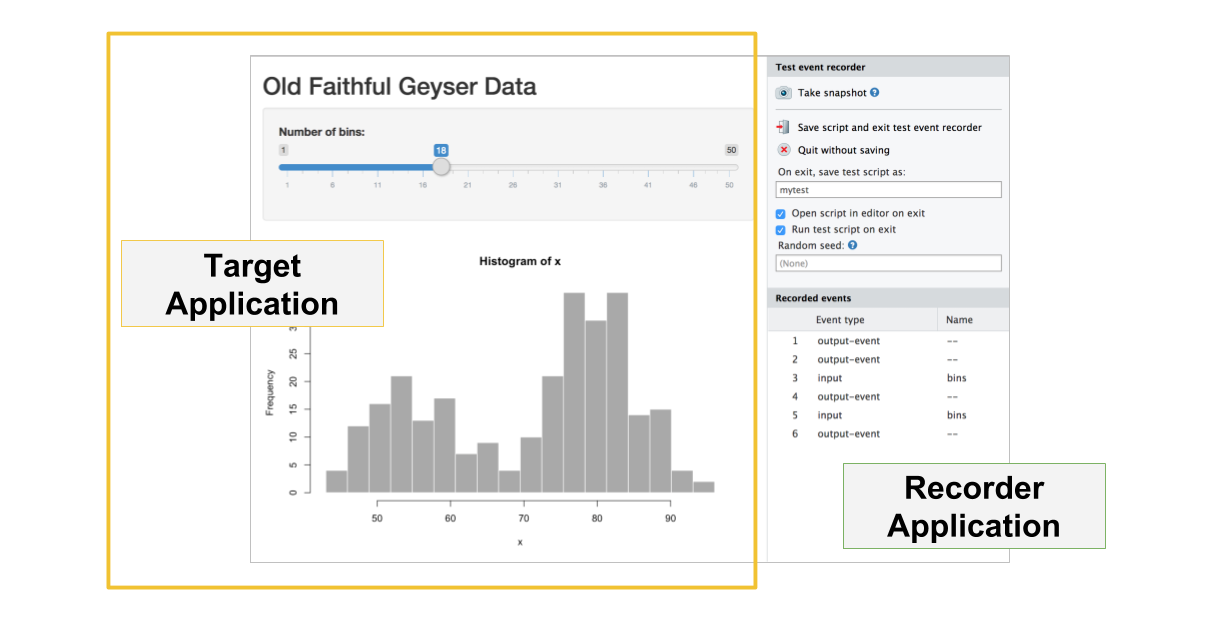
\includegraphics{imgs/testing/recorder_and_target.png}
\caption{Target and Recorder App iframe}
\end{figure}

The panel on the right displays some controls for the test recorder, as
well as a list of \textbf{recorded events}. As you interact with the
target app, you will see those interactions appear in the recorded
events list.

For testing a Shiny application, interacting with the inputs is only one
part of the equation. It's also necessary to check that the application
produces the correct outputs. This is accomplished by taking
\textbf{snapshots} of the application's state.

To take a snapshot of the application's state, click the \emph{Take
snapshot} button on the recorder app. This will record all input values,
output values, and exported values.

\textbf{Running Tests}

When you quit the test recorder, it will automatically run the test
script. There are three separate components involved in running tests:

\begin{enumerate}
\def\labelenumi{\arabic{enumi}.}
\tightlist
\item
  First is the \textbf{test driver}. This is the R process that
  coordiates the testing and controls the web browser. When working on
  creating tests interactively, this is the R process that you use.
\item
  Next is the \textbf{Shiny process}, also known as the \textbf{server}.
  This is the R process that runs the target Shiny application.
\item
  Finally, there is the \textbf{web browser}, also known as the
  \textbf{client}, which connects to the server. This is a headless web
  browser - one which renders the web page internally, but doesn't
  display the content to the screen (PhantomJS).
\end{enumerate}

So, when you exit the test recorder, it will by default automatically
run the test script and print something like this:

\begin{verbatim}
Saved test code to /path/to/app/tests/mytest.R
Running mytest.R 
====== Comparing mytest ...
  No existing snapshots at mytest-expected/. This is a first run of tests.

Updating baseline snapshot at tests/mytest-expected
Renaming tests/mytest-current
      => tests/mytest-expected.
\end{verbatim}

This is the result of running \texttt{testApp()}, which can also be
manually run by providing the desired application and test like this:

\texttt{testApp("exampleApp",\ "mytest")}

The built-in integreation with RStudio v1.2 provides \texttt{Run\ Tests}
as a drop down menu option in your Shiny app source file (see it located
under the \emph{Record Test} option in the screenshot above).

\textbf{Subsequent Test Runs}

After the initial test run, you can continue to run the tests to check
for changes in application behavior.

If there are any differences between current and expected results, the
test output will look something like this:

\begin{verbatim}
Running mytest.R 
====== Comparing mytest ...
  Differences detected between mytest-current/ and mytest-expected/:

    Name         Status      
    001.json  != Files differ
    001.png   != Files differ
Would you like to view the differences between expected and current results [y/n]? 
\end{verbatim}

To view failed tests in the RStudio IDE, go to the \emph{Build tab} and
make sure the \emph{issues toggle} is selected:

\begin{figure}
\centering
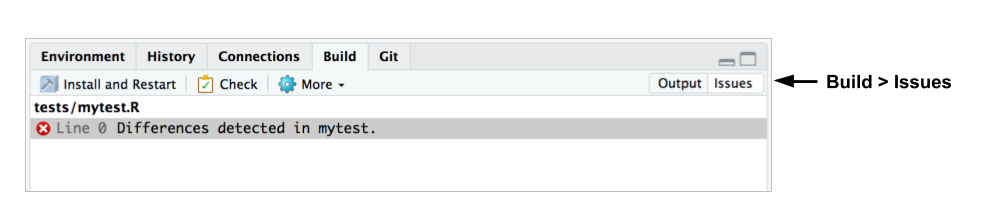
\includegraphics{imgs/testing/failed_tests.png}
\caption{View Failed Tests}
\end{figure}

For each test with different results, you can see the differences
between the expected and current results.

\textbf{Testing Code}

The \texttt{shinytest} package was created for testing Shiny
applications on the interaction-level. To test Shiny code and functions,
we suggest using the \texttt{testthat} package.

\href{http://testthat.r-lib.org/}{Info}
\href{https://github.com/r-lib/testthat}{GitHub}

Learn about testing and how to setup test workflow and structure:
\href{http://r-pkgs.had.co.nz/tests.html}{R packages by Hadley Wickham}

\hypertarget{workshop-exercise-shinytest}{%
\subsubsection{\texorpdfstring{Workshop Exercise:
\texttt{shinytest}}{Workshop Exercise: shinytest}}\label{workshop-exercise-shinytest}}

\textbf{First: Open app.R and use `Record Test'}

\textbf{Discussion:}

\emph{Understanding shinytest}

\begin{itemize}
\tightlist
\item
  What does the recording file create?
\item
  What challenges might our app pose to testing?
\item
  Can you run the tests and get a success?
\item
  How might you automate tests?
\end{itemize}

\textbf{Deliverable: Try \texttt{shinytest}}

\begin{itemize}
\tightlist
\item
  A set of tests that can catch unintentional changes to our app.
\end{itemize}

\hypertarget{profiling-the-most-important-thing}{%
\chapter{Profiling: ``The most important
thing''}\label{profiling-the-most-important-thing}}

Profvis is a tool for helping you to understand how R spends its time.
It provides a interactive graphical interface for visualizing data from
\texttt{Rprof}, R's built-in tool for collecting profiling data.

\begin{itemize}
\tightlist
\item
  \href{https://rstudio.github.io/profvis/}{Profvis Home}
\end{itemize}

To install profvis from CRAN: \texttt{install.packages("profvis")}

The RStudio IDE includes integrated support for profiling with profvis.
These features are available in the current Preview Release of RStudio.

\emph{Profvis: Profiling tools for faster R code}

\begin{itemize}
\tightlist
\item
  How do I make my R code faster?
\item
  Why is my R code slow?
\end{itemize}

\begin{figure}
\centering
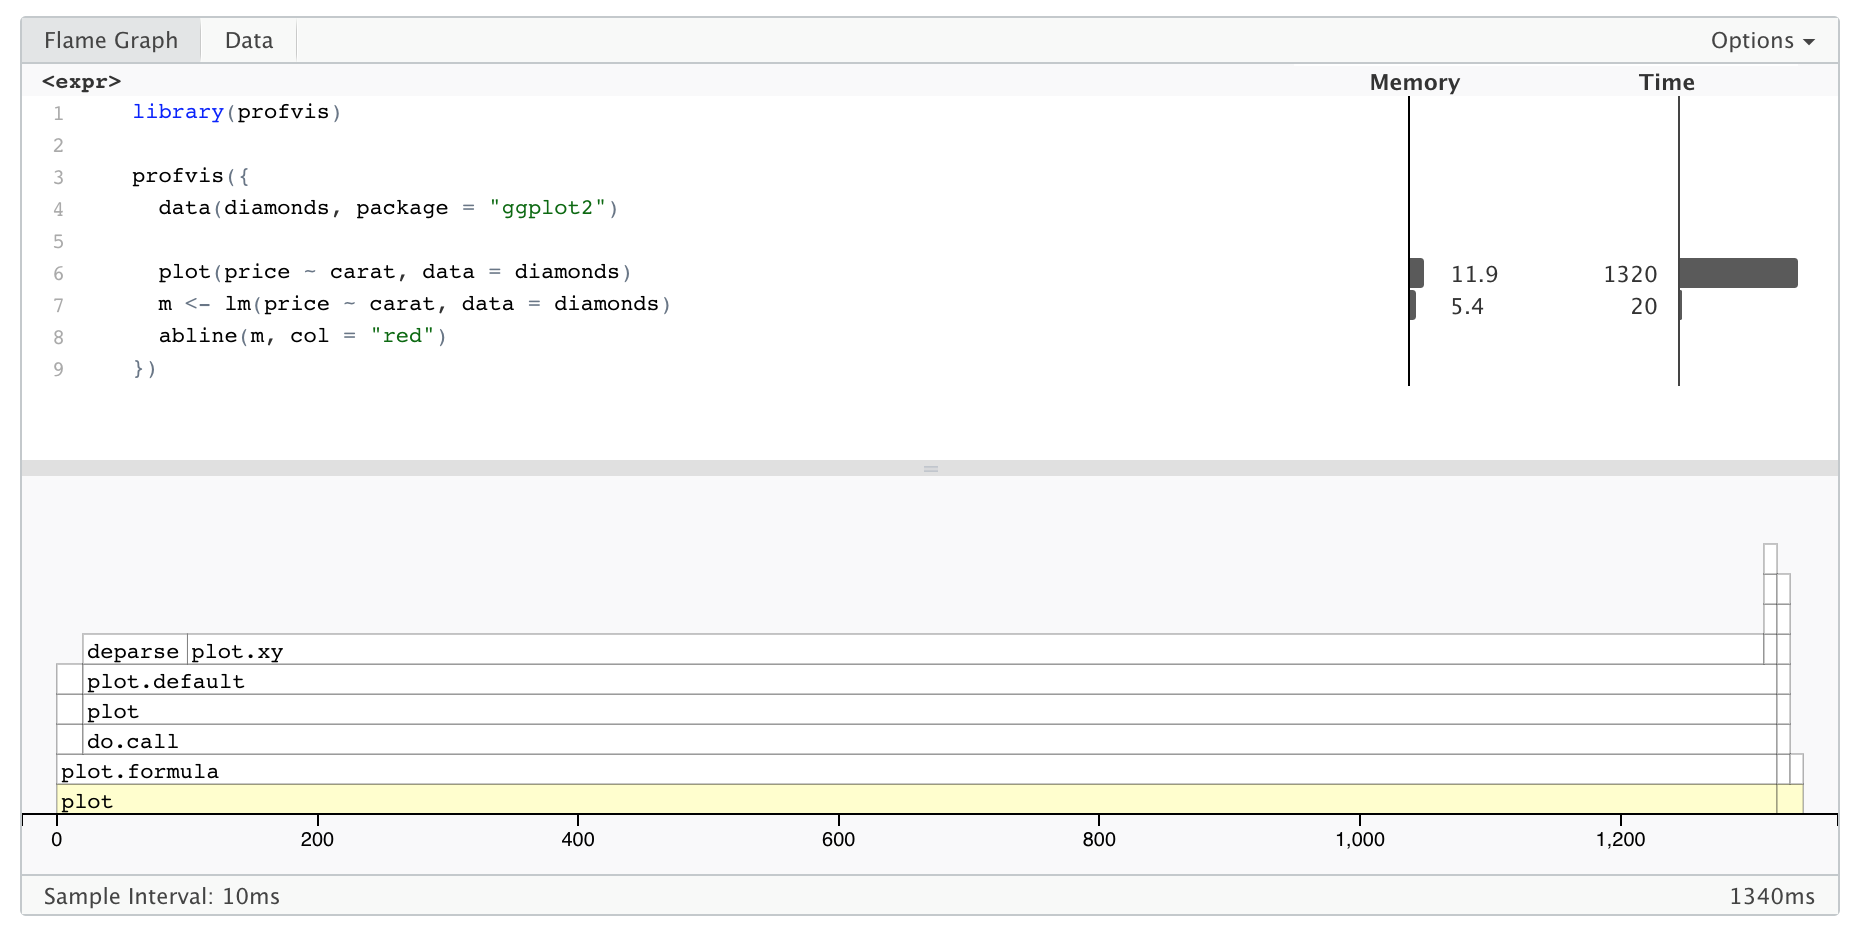
\includegraphics{imgs/profiling/use-profvis.png}
\caption{Profvis in Use}
\end{figure}

Each block in the flame graph represents a call to a function, or
possibly multiple calls to the same function. The width of the block is
proportional to the amount of time spent in that function. When a
function calls another function, another block is added on top of it in
the flame graph.

The profiling data has some limitations: some internal R functions don't
show up in the flame graph, and it offers no insight into code that's
implemented in languages other than R (e.g.~C, C++, or Fortran).

Profvis is interactive. You can try the following:

\begin{itemize}
\tightlist
\item
  As you mouse over the flame graph, information about each block will
  show in the info box.
\item
  Yellow flame graph blocks have corresponding lines of code on the
  left. (White blocks represent code where profvis doesn't have the
  source code -- for example, in base R and in R packages. But see this
  FAQ if you want package code to show up in the code panel.) If you
  mouse over a yellow block, the corresponding line of code will be
  highlighted. Note that the highlighted line of code is where the
  yellow function is called from, not the content of that function.
\item
  If you mouse over a line of code, all flame graph blocks that were
  called from that line will be highlighted.
\item
  Click on a block or line of code to lock the current highlighting.
  Click on the background, or again on that same item to unlock the
  highlighting. Click on another item to lock on that item.
\item
  Use the mouse scroll wheel or trackpad's scroll gesture to zoom in or
  out in the x direction.
\item
  Click and drag on the flame graph to pan up, down, left, right.
\item
  Double-click on the background to zoom the x axis to its original
  extent.
\item
  Double-click on a flamegraph block to zoom the x axis the width of
  that block.
\end{itemize}

\textbf{Things to remember:}

\begin{itemize}
\tightlist
\item
  Understand how the sampling profiler works
\item
  Understand the \texttt{profvis} interface
\item
  Sometimes performance bottlenecks are counterintuitive!
\end{itemize}

\hypertarget{workshop-exercise-profiling}{%
\subsubsection{Workshop Exercise:
Profiling}\label{workshop-exercise-profiling}}

\textbf{First: Create a profile of our app}

\textbf{Discussion:}

\emph{Understanding app performance}

\begin{itemize}
\tightlist
\item
  Where does our app spend most of its time?
\item
  Do any parts of the profile surprise you?
\item
  If you test the app again, do you get the same results?
\end{itemize}

\emph{Additional Group Discussion}

\begin{itemize}
\tightlist
\item
  Is the call to \texttt{gt} slow?
\item
  Why does \texttt{getStudentNum} take so much longer than
  \texttt{getStudentBin}? How could we speed this up?
\end{itemize}

\textbf{Deliverable: Optimization Recommendations}

\begin{itemize}
\tightlist
\item
  One recommendation for how we could speed up our app.
\end{itemize}

\hypertarget{references-and-resources}{%
\subsubsection{References and
Resources}\label{references-and-resources}}

\begin{itemize}
\tightlist
\item
  \href{https://tailrecursion.com/slides/fast-shiny/\#/title-slide}{Make
  Shiny Fast by Alan Dipert}
\item
  \href{https://github.com/rstudio/webinars/blob/master/26-Profiling/Profiling.pdf}{Profvis
  Webinar Slides}
\item
  \href{http://shiny.rstudio.com/articles/profiling.html}{Shiny Dev
  Center Article: Profiling your Shiny app}
\end{itemize}

\hypertarget{deployment}{%
\chapter{Deployment}\label{deployment}}

\hypertarget{rstudio-connect}{%
\section{RStudio Connect}\label{rstudio-connect}}

\begin{quote}
It doesn't matter how great your analysis is unless you can explain it
to others: you need to communicate your results. - Grolemund \& Wickham
in \emph{R For Data Science}
\end{quote}

\begin{figure}
\centering
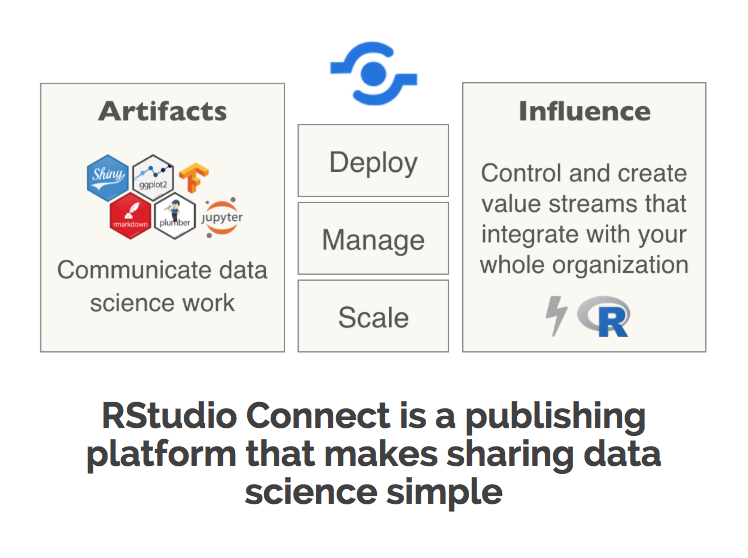
\includegraphics{imgs/deployment/rstudio-connect.png}
\caption{RStudio Connect}
\end{figure}

\hypertarget{workshop-exercise-inital-deployment}{%
\subsubsection{Workshop Exercise: Inital
Deployment}\label{workshop-exercise-inital-deployment}}

\textbf{First: Login to RStudio Connect}

\textbf{Discussion:}

\emph{Pre-deployment Brainstorm}

\begin{itemize}
\tightlist
\item
  What is our goal in deploying this code?
\item
  What does our code depend on locally?
\item
  What needs to deploy with our code?
\end{itemize}

\textbf{Deliverable: Deployed App}

Press the publish button in RStudio:

\begin{itemize}
\tightlist
\item
  Link to your Connect account
\item
  Select the files to publish (do NOT use the default to publish all the
  files)
\item
  Poke around at the results
\end{itemize}

\emph{Note: We are expecting an error!}

\begin{center}\rule{0.5\linewidth}{\linethickness}\end{center}

\hypertarget{packrat}{%
\section{Packrat}\label{packrat}}

\hypertarget{extended-topics-and-resources}{%
\section{Extended Topics and
Resources}\label{extended-topics-and-resources}}

\hypertarget{programmatic-deployment}{%
\subsection{Programmatic Deployment}\label{programmatic-deployment}}

\begin{itemize}
\tightlist
\item
  RStudio Connect
\end{itemize}

\hypertarget{collaborative-publishing}{%
\subsection{Collaborative Publishing}\label{collaborative-publishing}}

\begin{itemize}
\tightlist
\item
  RStudio Connect
\end{itemize}

\href{https://docs.rstudio.com/connect/user/publishing.html\#collaboration}{User
Guide Resource: Collaboration}

Some data products will have multiple authors and collaborators who are
responsible for managing the content deployed to RStudio Connect. The
first step to collaboration is sharing and working together on code. We
recommend using a version control tool like Git to coordinate
collaboration across many users.

\hypertarget{connecting-to-data-in-production}{%
\chapter{Connecting to Data in
Production}\label{connecting-to-data-in-production}}

\hypertarget{databases}{%
\subsubsection{Databases}\label{databases}}

\hypertarget{the-config-package}{%
\subsubsection{\texorpdfstring{The \texttt{config}
package}{The config package}}\label{the-config-package}}

\hypertarget{workshop-exercise-databases}{%
\subsubsection{Workshop Exercise:
Databases}\label{workshop-exercise-databases}}

\textbf{First: Read
\href{https://db.rstudio.com/best-practices/portable-code/}{This}!}

\textbf{Discussion:}

\emph{Data Management}

\begin{itemize}
\tightlist
\item
  How does your organization connect to data?
\item
  What data are we exposing to viewers? Is it appropriate for all
  viewers?
\item
  What else could we manage with the \texttt{config} package?
\end{itemize}

\textbf{Deliverable: Running, Deployed App}

\begin{itemize}
\tightlist
\item
  Update config.yml and Redeploy
\item
  Edit the Environment Variables in RStudio Connect
\end{itemize}

\hypertarget{revisit-the-deployment-checklist}{%
\subsubsection{Revisit the Deployment
Checklist}\label{revisit-the-deployment-checklist}}

\begin{figure}
\centering
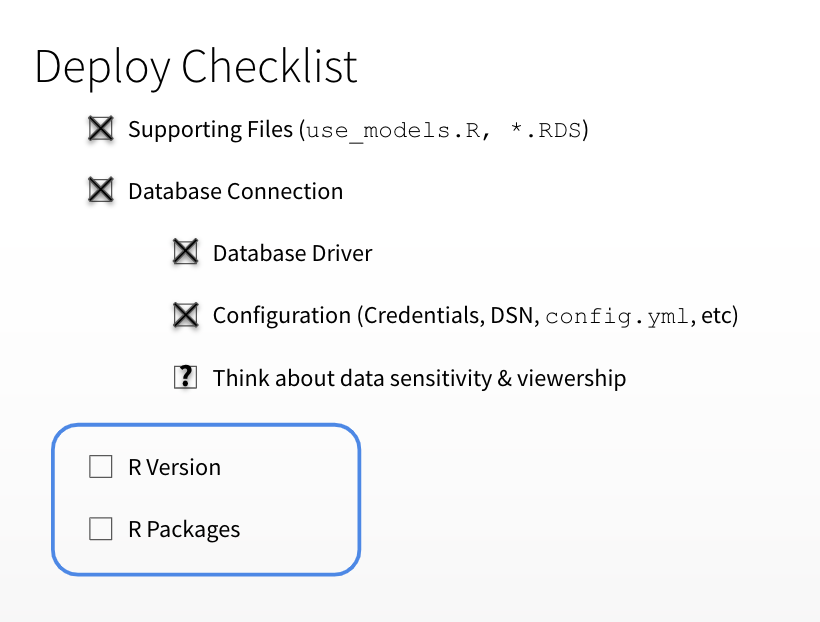
\includegraphics{imgs/databases/database-checklist.png}
\caption{Database Checklist}
\end{figure}

\hypertarget{load-testing}{%
\chapter{Load Testing}\label{load-testing}}

Load testing helps developers and administrators estimate how many users
their application can support. If an application requires tuning, load
testing and load test result analysis can be used to identify
performance bottlenecks and to guide changes to infrastructure,
configuration, or code.

It's a common misconception that \emph{``Shiny doesn't scale''}. In
actuality, properly-architected Shiny applications can be scaled
horizontally, a fact which Sean Lopp was recently able to demonstrate at
rstudio::conf 2018. We used \texttt{shinycannon} to simulate 10,000
concurrent users interacting with an application deployed to AWS. You
can see a recording of Sean's talk and the load test demonstration here:
\href{https://www.rstudio.com/resources/videos/scaling-shiny/}{Scaling
Shiny}

To perform a load test you'll need two pieces of software:
\texttt{shinyloadtest} and \texttt{shinycannon}.

\begin{itemize}
\tightlist
\item
  \texttt{shinyloadtest} is an R package used to generate recordings and
  analyze results. You should install it on your development machine.
  \href{https://github.com/rstudio/shinyloadtest}{GitHub}
\item
  \texttt{shinycannon} is the command-line replay tool. You can install
  it on your development machine for testing, but for best results we
  recommend installing it on a server, and preferably not the one the
  application under test is also on.
  \href{https://github.com/rstudio/shinycannon}{GitHub}
\end{itemize}

See the Load Testing Quickstart
\href{https://rstudio.github.io/shinyloadtest/\#quick-start}{Here}.

\hypertarget{optimization-loop-methodology}{%
\subsubsection{Optimization Loop
Methodology}\label{optimization-loop-methodology}}

\begin{itemize}
\tightlist
\item
  \textbf{Benchmark:} Use \texttt{shinyloadtest::record\_session()} to
  record interaction, \texttt{shinycannon} to simulate users
\item
  \textbf{Analyze:} Visualize and interpret the metrics
\item
  \textbf{Recommend:} Propose ways for the capacity of the application
  to be increased
\item
  \textbf{Optimize:} Implement recommendations and benchmark again.
  Repeat until satisfied
\end{itemize}

\emph{Workflow:}

\begin{figure}
\centering
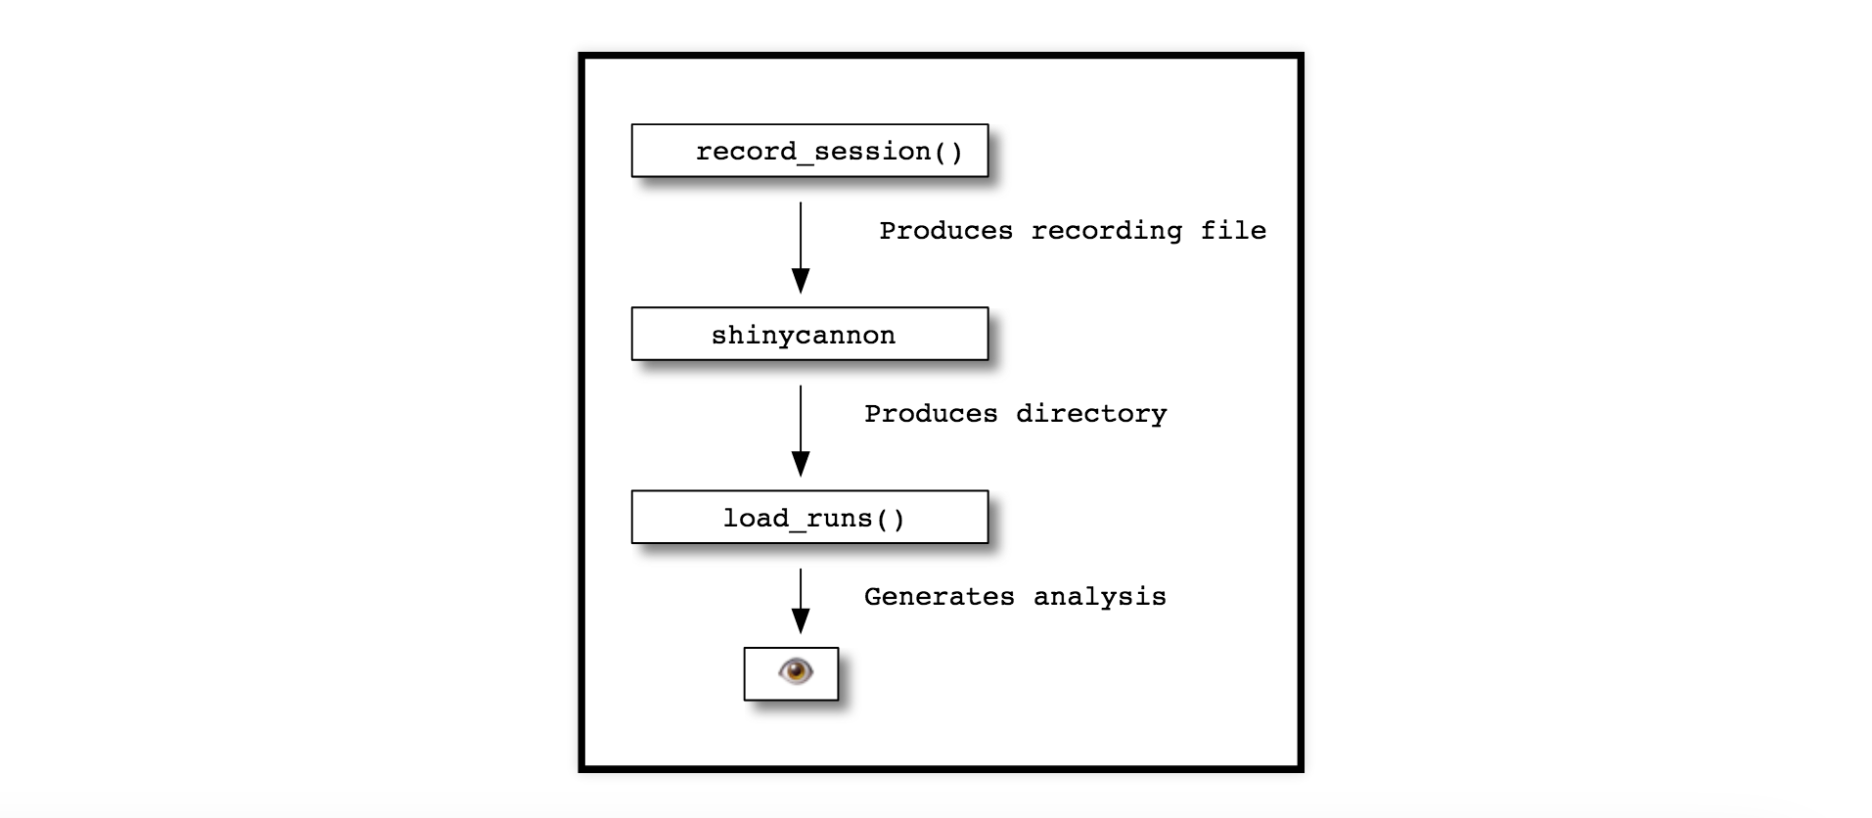
\includegraphics{imgs/loadtesting/loadtest-workflow.png}
\caption{Load Test Workflow}
\end{figure}

\begin{itemize}
\tightlist
\item
  Use `shinyloadtest to record a session with a Shiny app
\item
  Generate load with \texttt{shinycannon}
\item
  Analyze metrics with \texttt{shinyloadtest}
\item
  Make changes to the Shiny application
\item
  Generate load and analyze again
\end{itemize}

\begin{figure}
\centering
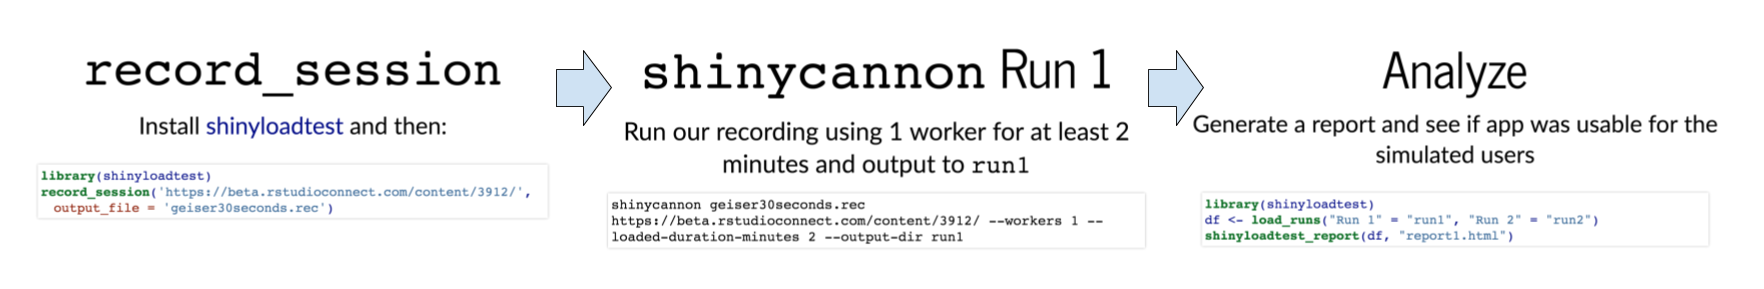
\includegraphics{imgs/loadtesting/loadtest-steps.png}
\caption{Load Test Steps}
\end{figure}

\href{https://rstudio.github.io/shinyloadtest/index.html}{Load Testing
Shiny Applications}

\hypertarget{workshop-exercise-load-testing}{%
\subsubsection{Workshop Exercise: Load
Testing}\label{workshop-exercise-load-testing}}

\textbf{First: Open runloadtest.R,do the pre-run checklist}

\textbf{Discussion:}

\emph{Preparing for the load test}

\begin{itemize}
\tightlist
\item
  First, what is up with the pre-run checklist? Any idea why these steps
  are (currently) necessary?
\item
  The \texttt{runloadtest.R} file is going to start with a baseline test
  of 1 and then a test of 25. Why is the baseline important?
\end{itemize}

\textbf{Deliverable: Run the load test}

\begin{itemize}
\tightlist
\item
  Follow the first set of commands in \texttt{runloadtest.R}
\item
  How did the experience for 1 user compare to the experience for 25
  users?
\end{itemize}

\hypertarget{references-and-resources-1}{%
\subsubsection{References and
Resources}\label{references-and-resources-1}}

\textbf{Webinar:}

\begin{itemize}
\tightlist
\item
  \href{https://resources.rstudio.com/webinars/load-testing-shiny-alan-dipert}{Load
  testing Shiny by Alan Dipert}
\item
  \href{https://github.com/rstudio/webinars/blob/master/63-shinyloadtest/slides.pdf}{Webinar
  Slides}
\end{itemize}

\textbf{Vignettes:}

\begin{itemize}
\tightlist
\item
  \href{https://rstudio.github.io/shinyloadtest/articles/analyzing-load-test-logs.html}{Analyzing
  Load Test Logs}
\item
  \href{https://rstudio.github.io/shinyloadtest/articles/case-study-scaling.html}{Case
  Study: Scaling an Application}
\item
  \href{https://rstudio.github.io/shinyloadtest/articles/limitations-of-shinyloadtest.html}{Limitations
  of \texttt{shinyloadtest}}
\item
  \href{https://rstudio.github.io/shinyloadtest/articles/load-testing-authenticated-apps.html}{Load
  Testing Authenticated Apps}
\end{itemize}

\hypertarget{plot-caching}{%
\chapter{Plot Caching}\label{plot-caching}}

\hypertarget{shiny-plot-caching-overview}{%
\section{Shiny Plot Caching
Overview}\label{shiny-plot-caching-overview}}

\href{https://resources.rstudio.com/rstudio-blog/shiny-1-2-0-plot-caching}{Blog:
Shiny 1.2.0: Plot caching - November 18, 2018}

The Shiny 1.2.0 package release introduced \emph{Plot Caching}, an
important new tool for improving performance and scalability in Shiny
applications.

\textbf{In a nutshell:} The term ``caching'' means that when
time-consuming operations are performed, we can save (cache) the results
so that the next time that operation is requested, instead of re-running
that calculation, we instead go fetch the previously cached result. When
applied appropriately, this ``fetch'' operation should take less time
that the original calculation and improve application performace (and
user experience) overall.

Shiny's reactive expressions do some amount of caching by default, and
you can use more explicit techniques to cache various data operations.
Examples include use of the \texttt{memoise} package, or manually saving
intermediate data frames to disk as CSV or RDS.

Plots are a very common and (potentially) expensive to compute type of
output object in Shiny applications, which makes them a great candidate
for caching. In theory, you could use \texttt{renderImage} to accomplish
this, but because Shiny's \texttt{renderPlot} function contains a lot of
complex infrastructure code, it's actually quite a difficult task.

Shiny v1.2.0 introduces a new function, \texttt{renderCachedPlot}, that
makes it much easiter to add plot caching to your application.

\hypertarget{when-to-use-plot-caching}{%
\subsection{When to use plot caching}\label{when-to-use-plot-caching}}

A shiny app is a good candidate for plot caching if:

\begin{enumerate}
\def\labelenumi{\arabic{enumi}.}
\tightlist
\item
  The app has plot outputs that are time-consuming to generate
\item
  These plots are a significant fraction of the total amount of time the
  app spends thinking
\item
  Most users are likely to request the same few plots
\end{enumerate}

\hypertarget{using-rendercachedplot}{%
\subsection{\texorpdfstring{Using
\texttt{renderCachedPlot}}{Using renderCachedPlot}}\label{using-rendercachedplot}}

\begin{figure}
\centering
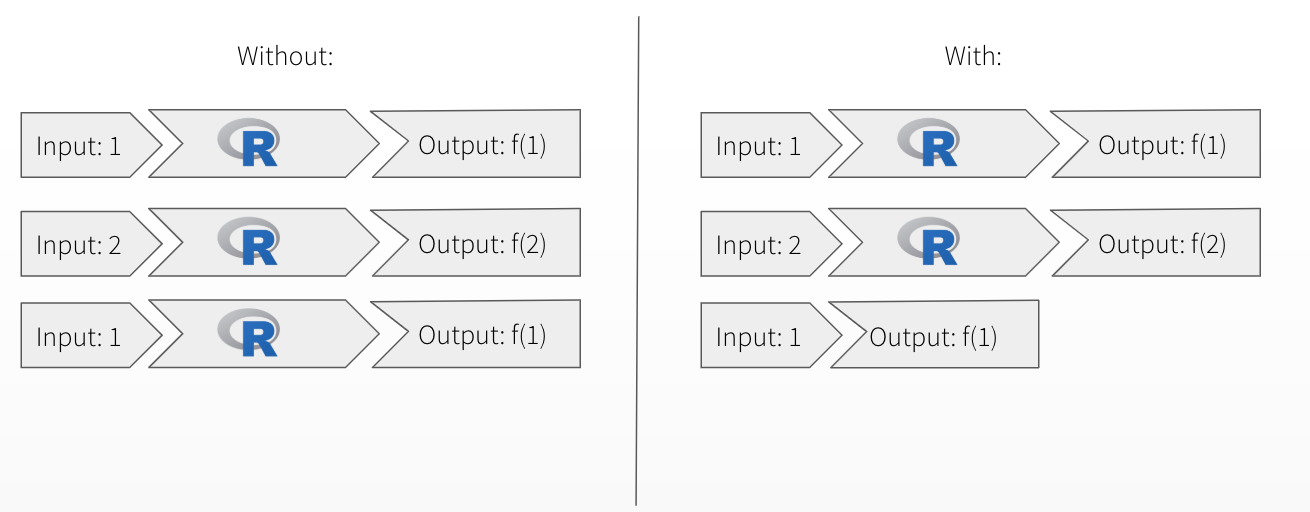
\includegraphics{imgs/plotcaching/rendercachedplot.png}
\caption{renderChachedPlot()}
\end{figure}

The following example is a simple, but computationally expensive, plot
output:

\begin{verbatim}
output$plot <- renderPlot({
  ggplot(diamonds, aes(carat, price, color = !!input$color_by)) +
    geom_point()
})
\end{verbatim}

The \texttt{diamonds} dataset has 53,940 rows. This plot might take
roughly 1580 milliseconds (1.58 seconds) to generate depending on the
resources available. For a high traffic Shiny application in production,
1.58 seconds is likely slower than ideal.

Plot caching can be implemented in two steps:

\begin{enumerate}
\def\labelenumi{\arabic{enumi}.}
\tightlist
\item
  Change \texttt{renderPlot} to \texttt{renderCachedPlot}
\item
  Provide a suitable \texttt{cacheKeyExpr}. This is an expression that
  Shiny will use to determine which invocations of
  \texttt{renderCachedPlot} should be considered equivalent to each
  other. In the example case, two plots with different
  \texttt{input\$color\_by} values can't be considered the ``same''
  plot, so the \texttt{cacheKeyExpr} needs to be
  \texttt{input\$color\_by}
\end{enumerate}

The example plot code would be updated like this:

\begin{verbatim}
output$plot <- renderCachedPlot({
  ggplot(diamonds, aes(carat, price, color = !!input$color_by)) +
    geom_point()
}, cacheKeyExpr = { input$color_by })
\end{verbatim}

With these code changes, the first time a plot with a particular
\texttt{input\$color\_by} is requested, it will take the normal amount
of time. But the next time it is requested, it will be almost instant,
as the previously rendered plot will be reused.

\hypertarget{workshop-exercise-plot-cache-benchmarking}{%
\subsection{Workshop Exercise: Plot cache
benchmarking}\label{workshop-exercise-plot-cache-benchmarking}}

\textbf{First: Update your app code to use \texttt{renderCachedPlot}}

\textbf{Discussion:} \emph{caching + shinyloadtest}

\begin{itemize}
\tightlist
\item
  How will introducing \texttt{renderCachedPlot} affect our load test
  experience?
\end{itemize}

\emph{What is the performance comparison between tests?}

\textbf{Deliverable: Re-run Load Test}

\begin{itemize}
\tightlist
\item
  Redeploy the version of the app with \texttt{renderCachedPlot}
\item
  Re-run the load test and compare the outputs (continue to follow along
  with \texttt{runloadtest.R})
\end{itemize}

\hypertarget{extended-topics-and-resources-1}{%
\subsection{Extended Topics and
Resources}\label{extended-topics-and-resources-1}}

\href{http://shiny.rstudio.com/articles/plot-caching.html}{Shiny
Article: Plot Caching by Winston Chang}

\hypertarget{plot-caching-on-rstudio-connect}{%
\subsubsection{Plot Caching on RStudio
Connect}\label{plot-caching-on-rstudio-connect}}

Shiny can store cached plots in memory, on disk, or with another backend
like \href{https://redis.io/}{Redis}. There are also a number of options
for limiting the size of the cache. Applications deployed on RStudio
Connect should use a disk cache and specify a subdirectory of the
application directory as the location for the cache. To do so, add this
code to the top of your application:

\begin{verbatim}
library(shiny)
shinyOptions(cache = diskCache("./cache"))
\end{verbatim}

This option ensures that cached plots will be saved and used across the
multiple R processes that RStudio Connect runs in support of an
application. In addition, this configuration results in the cache being
deleted and reset when new versions of the application are deployed.

\hypertarget{scaling}{%
\chapter{Scaling}\label{scaling}}

\hypertarget{application-scaling-101}{%
\section{Application Scaling 101}\label{application-scaling-101}}

\begin{figure}
\centering
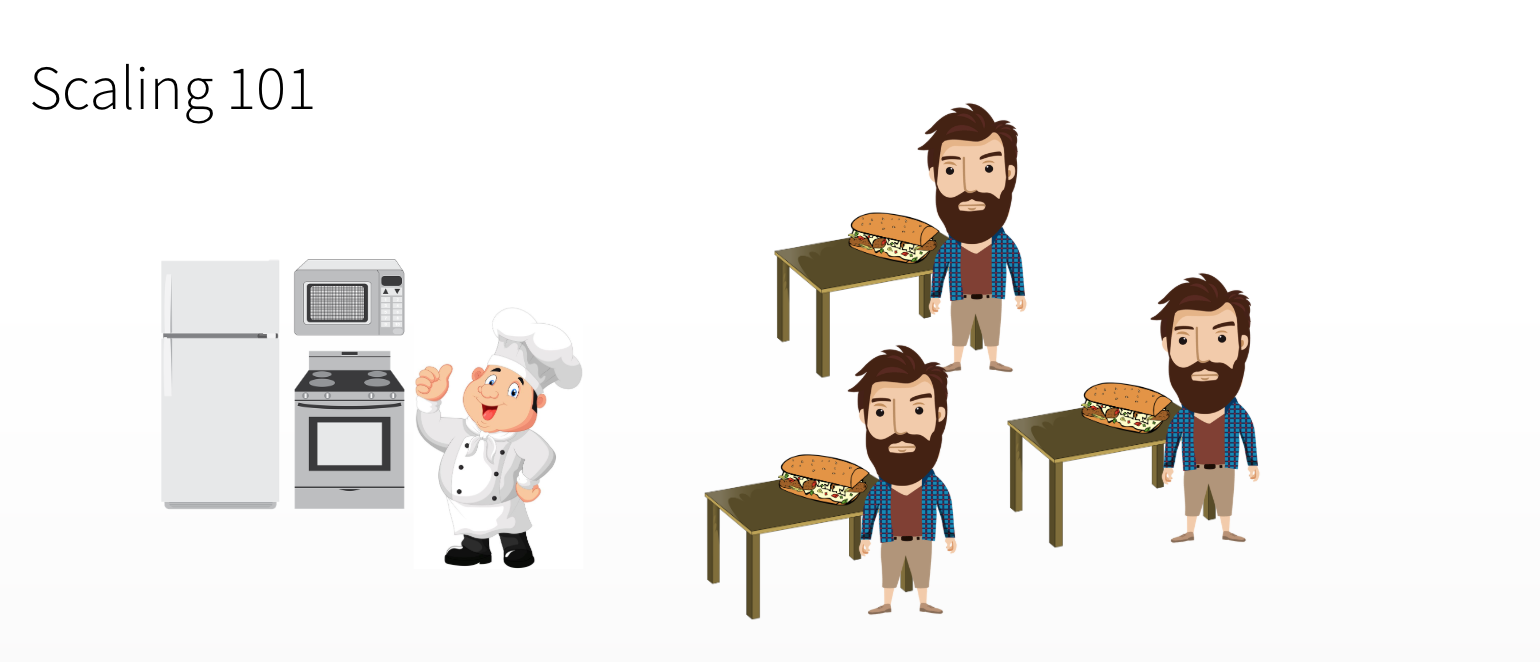
\includegraphics{imgs/scaling/kitchen-scaling.png}
\caption{Kitchen Scaling}
\end{figure}

\hypertarget{rstudio-connect-performance-settings}{%
\section{RStudio Connect Performance
Settings}\label{rstudio-connect-performance-settings}}

\textbf{Scaling and Performance Tuning in RStudio Connect}

\begin{itemize}
\tightlist
\item
  \href{https://support.rstudio.com/hc/en-us/articles/231874748-scaling-and-performance-tuning-rstudio-connect}{Article
  Reference}
\end{itemize}

RStudio Connect is built to scale content. Publishers and administrators
have access to runtime settings to help tune and scale their
applications and APIs. The primary concern for scaling content in
RStudio Connect is understanding when and how R code will be executed on
the server.

Content published on RStudio Connect can broadly fall into two
categories:

\begin{enumerate}
\def\labelenumi{\arabic{enumi}.}
\tightlist
\item
  Static / Batch Content
\end{enumerate}

Static content is content a user can visit without requiring a running
process. Examples include PDF documents, plots, and HTML files. HTML
files can include interactive elements where the interactivity occurs on
the client. RStudio Connect is able to update static content on a
schedule.

\begin{enumerate}
\def\labelenumi{\arabic{enumi}.}
\setcounter{enumi}{1}
\tightlist
\item
  Interactive Content
\end{enumerate}

A powerful component of RStudio Connect is the ability to host data
products that require backend processes during a user's visit. Examples
include shiny applications and R Markdown documents with runtime::shiny,
plumber APIs, and TensorFlow APIs. In the case of Shiny, an end user's
browser (the client) is connected with an R process running on the
server. When a user changes an input, the client sends a message to the
server and a portion of R code is re-run. The server sends back the
result as output. In the case of APIs, a client makes a request which is
sent to a running process, and the results are sent back to the client.

For Interactive Content, RStudio Connect enables scaling through
parameters that determine the content's
\href{https://docs.rstudio.com/connect/admin/appendix-configuration.html\#appendix-configuration-scheduler}{scheduler}.

\hypertarget{content-scheduler}{%
\subsection{Content Scheduler}\label{content-scheduler}}

When a user requests content with Shiny components, RStudio Connect
opens a channel between the user and an R process. Now, suppose a second
user requests the same content. There are two potential scenarios:

\begin{figure}
\centering
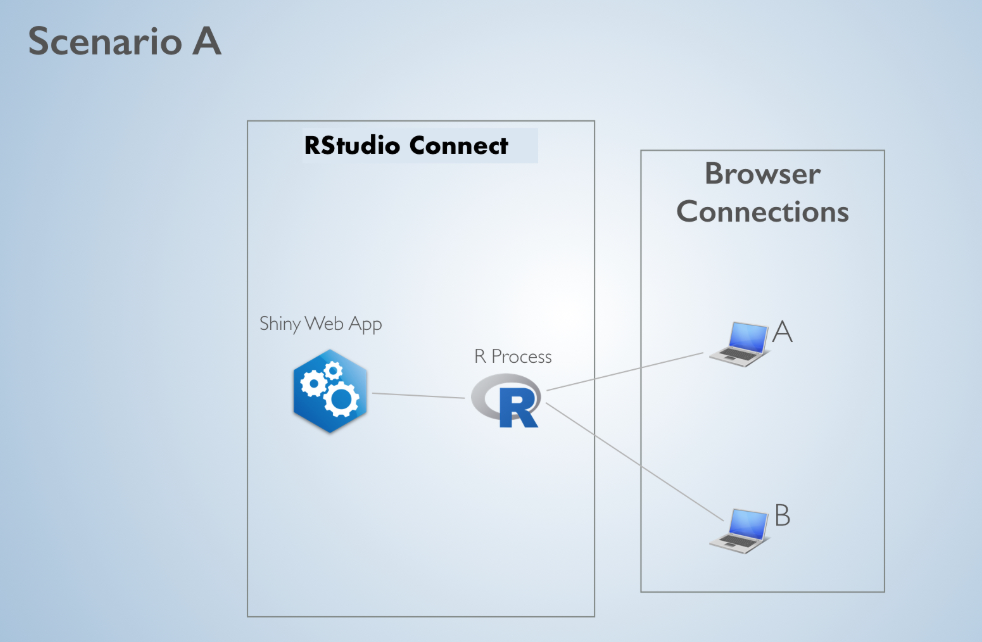
\includegraphics{imgs/scaling/scaling-a.png}
\caption{Scaling A}
\end{figure}

In Scenario A, both users are linked to the same R process. Because R is
single-threaded, if user A and user B both change an input and trigger R
calculations, their requests will be handled sequentially. (User B will
have to wait for user A's calculation to complete, and then for their
own calculation to complete before they will see an updated output).

\begin{figure}
\centering
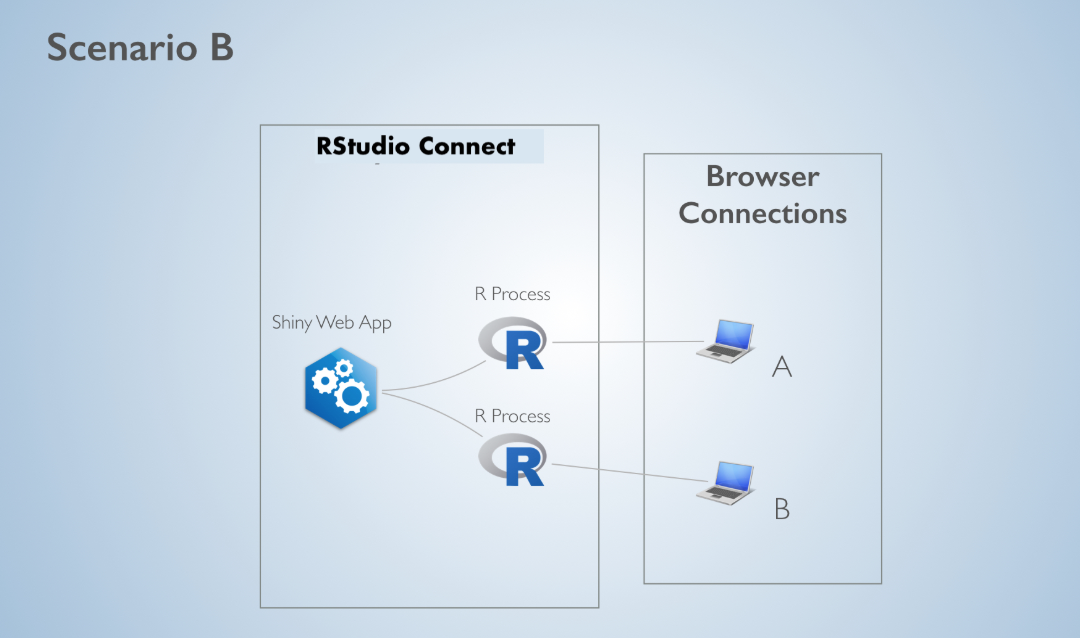
\includegraphics{imgs/scaling/scaling-b.png}
\caption{Scaling B}
\end{figure}

In Scenario B, Connect will link each user to their own R process. If
user A and user B both change an input, their calculations will happen
simultaneously.

Why wouldn't RStudio Connect always select Scenario B? The answer has to
do with memory and initial load time. When 2 users are connected to the
same R process, they get to share everything that is loaded outside of
the server function.

To see this, consider when the different pieces of Shiny application
code are executed:

\begin{figure}
\centering
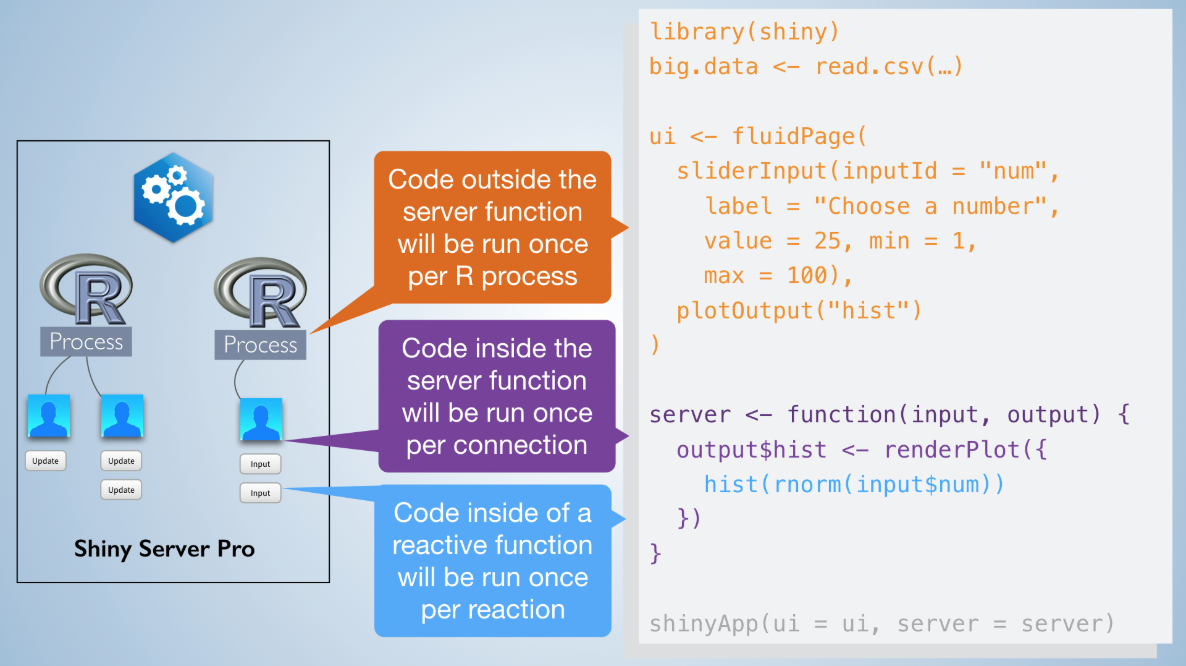
\includegraphics{imgs/scaling/app-execution.png}
\caption{App Execution}
\end{figure}

This works because Shiny makes use of R's unique scoping rules (read
more \href{http://shiny.rstudio.com/articles/scoping.html}{here}). In
Scenario B, all of the shiny code has to be re-run, including loading
any globally available data. This means the memory usage is 2x what it
would be in Scenario A. Additionally, spinning up an R process and
executing all of the shiny code takes time. While the application is
more responsive to both users after the web page is loaded, it will take
longer for them to connect initially.

The scheduling parameters tell RStudio Connect to act somewhere in
between Scenario A and Scenario B, to maximize the trade-off between app
responsiveness and memory consumption/load time. The parameters also
specify how long R processes and user connections should remain idle
before timing out.

\hypertarget{scheduling-parameters}{%
\subsection{Scheduling Parameters}\label{scheduling-parameters}}

\textbf{Max processes} - Determines the maximum number of processes that
will be created. Max processes x Max connections per process = total
number of concurrent connections. Default value is 3.

\emph{Pick a value that will support the expected number of concurrent
users or requests.}

\textbf{Min processes} - Determines the minimum number of processes that
will always be running. For Shiny applications and plumber APIs, user
requests only execute specific functions. R code outside of those
functions can be run when the process starts before user requests are
made, which can dramatically speed up response time.

\emph{Pick a number close to Max processes if your application or API
pre-loads a large amount of data to be shared by every user. Pick a
small number to minimize the amount of memory consumed.}

\textbf{Max connections per process} - The maximum number of connections
per process. Default value is 20.

\emph{Pick a small number if your content involves heavy computation.
Pick a larger number if your content shares data between users.
(e.g.~Pick a large number if your content takes a long time to load, but
after loading is very fast.)}

\textbf{Load factor} - Determines how aggressively new processes will be
created. A value close to 0 means new processes will be spun up
aggressively to try and keep the number of connections per process
small. A value close to 1 means the number of connections per process
will be close to max connections. Default value is 0.5.

\emph{Pick a small number if your content loads quickly but involves
expensive computation. Pick a number closer to 1 if your content loads
slowly, but after loading is fast OR if you want to minimize the amount
of memory.}

\hypertarget{workshop-exercise-1}{%
\subsubsection{Workshop Exercise 1}\label{workshop-exercise-1}}

\textbf{First: Open the runtime settings for your app}

\textbf{Discussion:}

\begin{itemize}
\tightlist
\item
  What do each of the settings mean?
\item
  What changes to the settings might affect our app?
\end{itemize}

\textbf{Deliverable: Re-run Load Test}

Test your hypothesis by changing the runtime settings and then re-run
the load test. Compare the results to the prior test (continue to follow
along with \texttt{runloadtest.R})

\hypertarget{workshop-exercise-2}{%
\subsubsection{Workshop Exercise 2}\label{workshop-exercise-2}}

\textbf{First: Open the admin dashboard in RStudio Connect}

\textbf{Discussion:}

\emph{Multi-Tenant Environment}

\begin{itemize}
\tightlist
\item
  What are the tradeoffs for modifying the scaling settings?
\item
  What else might you need to consider when sharing infrastructure?
\item
  How does these concerns change over time?
\end{itemize}

\textbf{Deliverable: Update checklist}

Create one pre-deployment checklist step and one every-2-months
checklist step based on your discussion.

\hypertarget{high-availability-and-horizontal-scaling}{%
\subsection{High Availability and Horizontal
Scaling}\label{high-availability-and-horizontal-scaling}}

Other considerations for widely accessed content are high availability
and horizontal scaling. Both require content to be hosted by more than
one server. RStudio Connect supports a
\href{https://docs.rstudio.com/connect/admin/high-availability.html}{cluster
setup}.

\hypertarget{r-markdown-documents-with-runtimeshiny}{%
\subsection{R Markdown Documents with
runtime::shiny}\label{r-markdown-documents-with-runtimeshiny}}

R Markdown documents are a bit different. In essence, an Rmd with
runtime::shiny specified places everything (data loading, UI creation,
etc) inside of the server function. The implication is an Rmd with
runtime::shiny will always consume more memory as users connect.

\href{https://rmarkdown.rstudio.com/authoring_shiny_prerendered.html}{Prerendered
Shiny Documents} alleviate this problem.

\hypertarget{devops-philosophy-tooling}{%
\chapter{DevOps Philosophy \& Tooling}\label{devops-philosophy-tooling}}

DevOps is a self-help philosophy for IT and software development teams
that work together. It seeks to address a core problem: \textbf{The Fear
of Taking Code into Production}

The whole point of this workshop is to get you some experience with what
it takes to get Shiny Applications running in

\begin{itemize}
\tightlist
\item
  Deployments/releases are high-risk events
\item
  It takes a long time to deliver new features to customers
\item
  There is no visibility into how code is deployed into production,
  therefore it is impossible to know what to optimize or fix in the
  system and/or people who seek to improve portions of workflow are
  likely not addressing true bottlenecks.
\item
  Dev and Ops have seemingly conflicting goals and objectives
\end{itemize}

The Fix (ref: The DevOps Handbook) ``The principles underpinning
DevOps'':

\begin{enumerate}
\def\labelenumi{\arabic{enumi}.}
\tightlist
\item
  Accelerate the delivery of work from Development to Operations to
  customers
\item
  Commit to evolving ever safer systems of work through feedback
\item
  Promote a high-trust culture and embrace continual learning and
  experimentation (risk-taking) in daily work
\end{enumerate}

\begin{center}\rule{0.5\linewidth}{\linethickness}\end{center}

\textbf{Flow}

\begin{itemize}
\tightlist
\item
  Make work visible
\item
  Limit Work in Progress (WIP)
\item
  Reduce Batch Sizes
\item
  Reduce the number of handoffs
\item
  Continually identify and elevate constraints
\item
  Eliminate hardships and waste in the value stream
\end{itemize}

Typical DevOps Transformation (pg. 22) - Environment creation - Code
Deployment - Test setup and run - Overly tight architechture

\textbf{Feedback}

\begin{itemize}
\tightlist
\item
  Working safely within complex systems

  \begin{itemize}
  \tightlist
  \item
    Complex work is managed so that problems in design and operations
    are revealed
  \item
    Problems are swarmed and solved
  \item
    New local knowledge is exploited globally throughout the
    organization
  \item
    Leaders create leaders
  \end{itemize}
\item
  See problems as they occur
\item
  Swarm and solve problems to build new knowledge
\item
  Keep pushing quality closer to the source
\item
  Enable optimizing for downstream work centers
\end{itemize}

\textbf{Continual Learning \& Experimentation}

\begin{itemize}
\tightlist
\item
  Enable organizational learning and a safety culture
\item
  Institutionalize the improvement of daily work
\item
  Transform local discoveries into global improvements
\item
  Inject resilience patterns into daily work
\end{itemize}

Generative organizations (pg. 39) // What type of organization do you
have? Comparison Activity - Information is actively sought - Messengers
are trained - Responsibilities are shared - Bridging between teams is
rewarded - Failure causes inquiry - New ideas are welcomed

\begin{quote}
Even more important than daily work is the improvement of daily work
--Mike Orzen, Lean IT
\end{quote}

\hypertarget{devops-vocab-101}{%
\subsubsection{DevOps Vocab 101}\label{devops-vocab-101}}

Deployment Lead Time

Hardships and Waste: - Partially done work - Extra processes - Extra
features - Task switching - Waiting - Motion - Defects - Nonstandard or
manual work - Heroics

\hypertarget{integrating-data-science-and-devops}{%
\subsubsection{Integrating Data Science and
DevOps}\label{integrating-data-science-and-devops}}

\hypertarget{how-does-data-science-fit-in-with-the-devops-philosophy}{%
\paragraph{How does data science fit in with the DevOps
philosophy?}\label{how-does-data-science-fit-in-with-the-devops-philosophy}}

It's not \emph{your job} to understand operations and systems
administration. And it's not IT's job to understand R programming and
shiny app development. But it takes shared goals and a little empathy
from both sides to get less painful results.

We can leverage (steal) the DevOps philosophy and apply it to manage
code deployment handoffs between data science and IT.

Foundations:

What do your dev, test and production environments look like? - Do
developers have access to production-like environments on their own
workstations? - Can these evnvironments be assembled on-demand? -
Version Control - Infrastructure as Code

\hypertarget{design-and-management-of-analytic-infrastructure-alternative-architectures}{%
\paragraph{Design and Management of Analytic Infrastructure (alternative
architectures)}\label{design-and-management-of-analytic-infrastructure-alternative-architectures}}

\hypertarget{programatic-deployment-into-rstudio-connect}{%
\paragraph{Programatic Deployment into RStudio
Connect}\label{programatic-deployment-into-rstudio-connect}}

\hypertarget{deployment-release-patterns}{%
\paragraph{Deployment Release
Patterns}\label{deployment-release-patterns}}

\begin{itemize}
\tightlist
\item
  Environment based release patterns
\item
  Application based release patterns
\end{itemize}

\hypertarget{feature-toggles-dark-launch}{%
\subsubsection{Feature Toggles (Dark
Launch)}\label{feature-toggles-dark-launch}}

\hypertarget{user-meta-data}{%
\paragraph{User meta-data}\label{user-meta-data}}

Shiny applications can access the username and groups of the current
user through the session parameter of the shinyServer function.

Groups meta-data is populated when using password, or OAuth
authentication. It is not populated with LDAP, PAM, or proxy
authentication.

\begin{verbatim}
shinyServer(function(input, output, session) {
  output$username <- reactive({
    session$user
  })
  
  output$groups <- reactive({
    session$groups
  })
})
\end{verbatim}

Your application could use this information to display customized
messages or to enable functionality for a specific subset of users.

\hypertarget{extended-topics-resources}{%
\subsubsection{Extended Topics \&
Resources}\label{extended-topics-resources}}

\textbf{Shiny Application Usage (Instrumentation)}

RStudio Connect exposes usage information about shiny applications that
will tell you which ones have been used, by whom and for how long. It is
available via an API that may be used by administrators or publishers.
Publishers may retrieve information about their own applications only.

More information about using the API is included in the historical
information chapter of the RStudio Connect Admin Guide.

\hypertarget{production-case-studies}{%
\chapter{Production Case Studies}\label{production-case-studies}}

\emph{Workshop Exercise: Case Study Discussions}

\textbf{First: Pick one case study}

\textbf{Discuss:}

\begin{itemize}
\tightlist
\item
  What tools does your admin team use?
\item
  How would you explain the goals of a shiny app to DevOps?
\end{itemize}

\textbf{Deliverable:}

\begin{itemize}
\tightlist
\item
  Whiteboard (in a medium of your choice) what an architecture might
  look like for your case study.
\item
  Delineate who (and what tool) is responsible for code, R, R packages.
\end{itemize}

\hypertarget{case-study-a-devtestprod}{%
\subsubsection{Case Study A:
Dev/Test/Prod}\label{case-study-a-devtestprod}}

Before publishing an update to our app, we want to run user acceptance
tests.

\begin{figure}
\centering
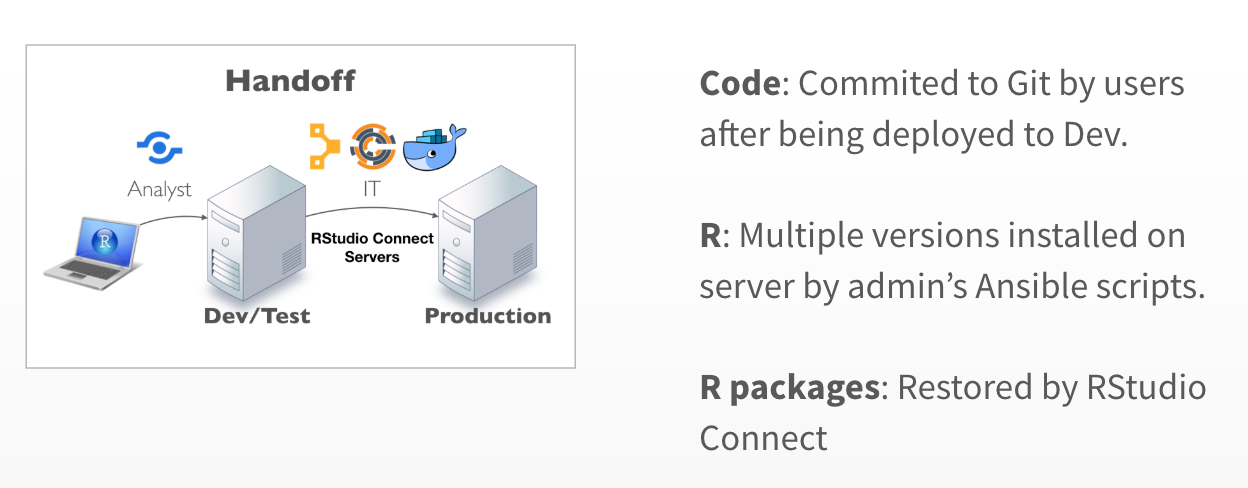
\includegraphics{imgs/case-studies/case-a.png}
\caption{Case A Considerations}
\end{figure}

\hypertarget{case-study-b-ci-git-chef}{%
\subsubsection{Case Study B: CI, Git,
Chef}\label{case-study-b-ci-git-chef}}

All of our production code must be deployed from Git.

\begin{figure}
\centering
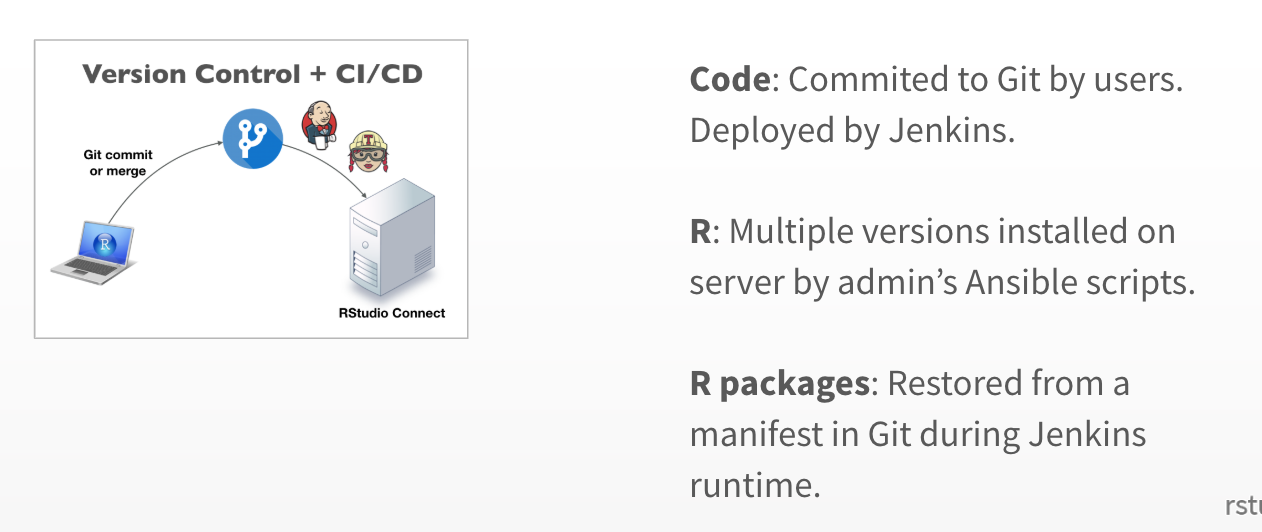
\includegraphics{imgs/case-studies/case-b.png}
\caption{Case B Considerations}
\end{figure}

\hypertarget{case-study-c-docker}{%
\subsubsection{Case Study C: Docker}\label{case-study-c-docker}}

We scale applications through Docker - how does Shiny fit in?

\begin{figure}
\centering
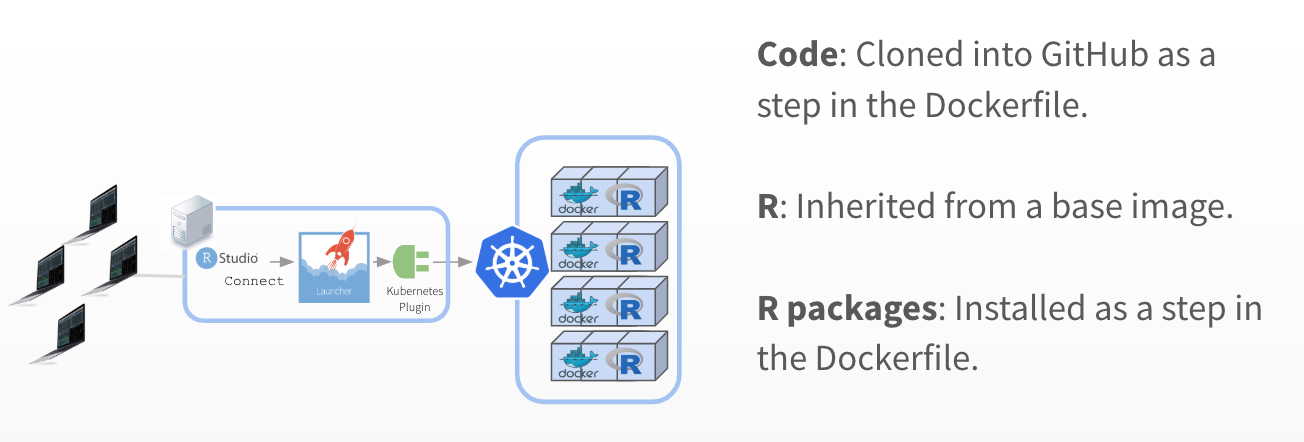
\includegraphics{imgs/case-studies/case-c.png}
\caption{Case C Considerations}
\end{figure}

\hypertarget{alternatives-to-shiny}{%
\chapter{Alternatives to Shiny}\label{alternatives-to-shiny}}

\hypertarget{plumber}{%
\section{Plumber}\label{plumber}}

\emph{Could our student ``scoring'' be hosted outside of the Shiny app?}

\begin{figure}
\centering
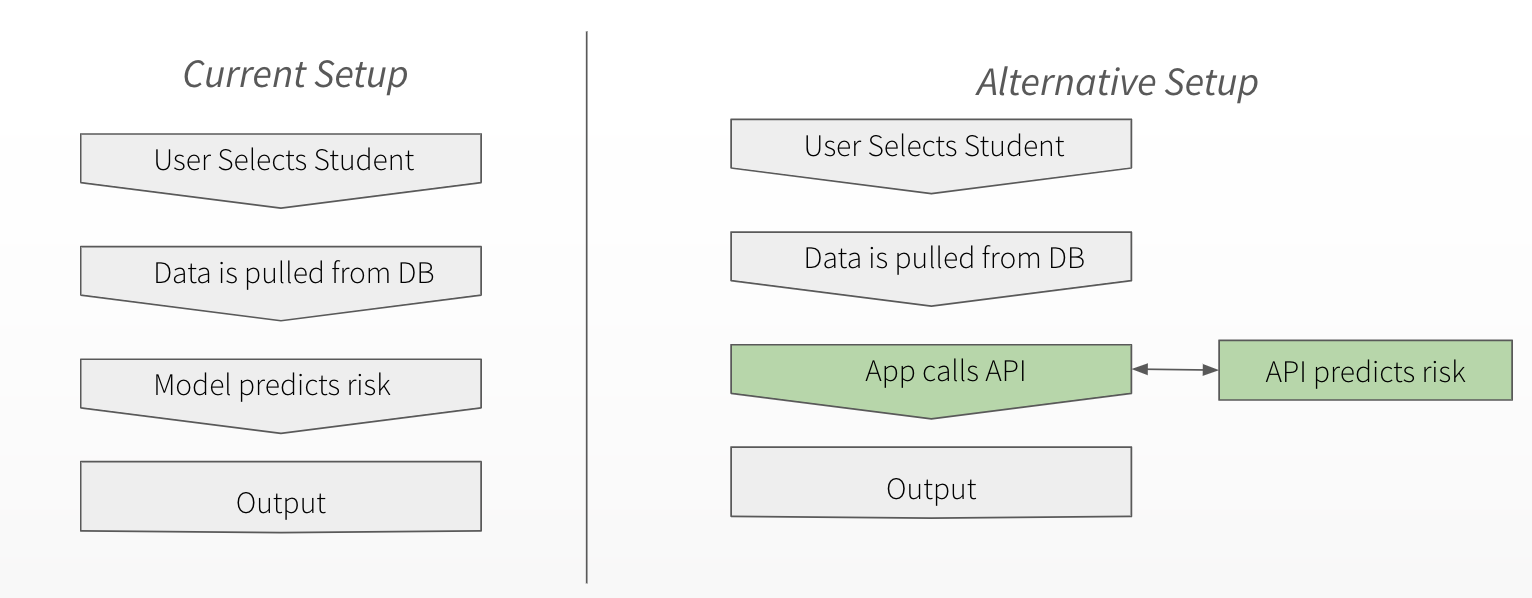
\includegraphics{imgs/shiny-alt/plumber-alt.png}
\caption{Plumber Scoring}
\end{figure}

\hypertarget{intro-to-plumber}{%
\subsection{Intro to Plumber}\label{intro-to-plumber}}

\textbf{Resources:}

Plumber is an R package that converts your existing R code to a web API
using a handful of special one-line comments.

\begin{quote}
What are Web APIs? For some, APIs (Application Programming Interface)
are things heard of but seldom seen. However, whether seen or unseen,
APIs are part of everyday digital life. In fact, you've likely used a
web API from within R, even if you didn't recognize it at the time!
Several R packages are simply wrappers around popular web APIs, such as
\texttt{tidycensus} and \texttt{gh}. Web APIs are a framework for
sharing information across a network, most commonly through HTTP.
\end{quote}

You can install the latest stable version from CRAN using the following
command:

\begin{verbatim}
install.packages("plumber")
\end{verbatim}

These comments allow plumber to make your R functions available as API
endpoints. You can either prefix the comments with \texttt{\#*} or
\texttt{\#\textquotesingle{}} but we recommend the former since
\texttt{\#\textquotesingle{}} will conflict with the Roxygen package.

Basic example:

\begin{enumerate}
\def\labelenumi{\arabic{enumi}.}
\tightlist
\item
  Create a File: \texttt{plumber.R}
\end{enumerate}

\begin{verbatim}
# plumber.R

#* Echo back the input
#* @param msg The message to echo
#* @get /echo
function(msg=""){
  list(msg = paste0("The message is: '", msg, "'"))
}

#* Plot a histogram
#* @png
#* @get /plot
function(){
  rand <- rnorm(100)
  hist(rand)
}

#* Return the sum of two numbers
#* @param a The first number to add
#* @param b The second number to add
#* @post /sum
function(a, b){
  as.numeric(a) + as.numeric(b)
}
\end{verbatim}

\begin{enumerate}
\def\labelenumi{\arabic{enumi}.}
\setcounter{enumi}{1}
\tightlist
\item
  Serve the \texttt{plumber.R} file from the R console:
\end{enumerate}

\begin{verbatim}
library(plumber)
r <- plumb("plumber.R")  # Where 'plumber.R' is the location of the file shown above
r$run(port=8000)
\end{verbatim}

You can visit this URL using a browser or a terminal to run your R
function and get the results. For instance
\url{http://localhost:8000/plot} will show you a histogram, and
\url{http://localhost:8000/echo?msg=hello} will echo back the `hello'
message you provided.

\begin{enumerate}
\def\labelenumi{\arabic{enumi}.}
\setcounter{enumi}{2}
\tightlist
\item
  Hit the endpoints (example: use \texttt{curl} from mac/linux terminal)
\end{enumerate}

\begin{verbatim}
$ curl "http://localhost:8000/echo"
 {"msg":["The message is: ''"]}
 
$ curl "http://localhost:8000/echo?msg=hello"
 {"msg":["The message is: 'hello'"]}
 
$ curl --data "a=4&b=3" "http://localhost:8000/sum"
 [7]
\end{verbatim}

\hypertarget{references-and-resources-2}{%
\subsubsection{References and
Resources}\label{references-and-resources-2}}

\begin{itemize}
\tightlist
\item
  \href{https://www.rplumber.io/}{Reference: Plumber Docs}
\item
  \href{https://blog.rstudio.com/2018/10/23/rstudio-1-2-preview-plumber-integration/}{Plumber
  Integration in RStudio 1.2}
\item
  \href{https://rviews.rstudio.com/2018/07/23/rest-apis-and-plumber/}{RViews
  Blog: REST APIs and Plumber by James Blair}
\item
  \href{https://www.rstudio.com/resources/videos/plumber-turning-your-r-code-into-an-api/}{Video:
  Turning your R code into an API by Jeff Allen}
\item
  \href{https://www.rstudio.com/resources/videos/plumbing-apis-with-plumber/}{Webinar:
  Plumbing APIs with Plumber by Jeff Allen}
\end{itemize}

\hypertarget{workshop-exercise-plumber}{%
\subsection{Workshop Exercise:
Plumber}\label{workshop-exercise-plumber}}

\textbf{First: Try creating your own plumber API in the IDE (New File)}

\textbf{Discussion:}

\emph{Consider our new architecture}

Does my R functionality need to be accessed by other systems?

\begin{itemize}
\tightlist
\item
  Why might a RESTful API be easier to scale than a Shiny app?

  \begin{itemize}
  \tightlist
  \item
    Requests are stateless, so it is easier for R processes to come and
    go.
  \end{itemize}
\item
  What benefits come from pulling the modeling code out of our app?

  \begin{itemize}
  \tightlist
  \item
    We can update the model independently of the app, e.g.~if we wanted
    to retrain.
  \end{itemize}
\end{itemize}

\textbf{Deliverable:}

\begin{itemize}
\tightlist
\item
  Add an item to our production checklist to consider plumber.
\item
  Add 2 decision criteria to the checklist to decide when a plumber API
  would be useful.
\end{itemize}

\hypertarget{r-markdown}{%
\section{R Markdown}\label{r-markdown}}

R Markdown is an open-source R package that turns your analyses into
high quality documents, reports, presentations and dashboards. An R
Markdown document is written in markdown (an easy-to-write plain text
format) and contains chunks of embedded R code. R Markdown documents are
fully reproducible and support dozens of output formats including HTML,
PDF, and Microsoft Word documents.

R Markdown files are designed to be used with the \texttt{rmarkdown}
package. \texttt{rmarkdown} comes installed with the RStudio IDE, but
you can acquire your own copy of \texttt{rmarkdown} from CRAN with the
command:

\begin{verbatim}
install.packages("rmarkdown")
\end{verbatim}

R Markdown reports rely on three frameworks:

\begin{enumerate}
\def\labelenumi{\arabic{enumi}.}
\tightlist
\item
  \texttt{markdown} for formatted text
\item
  \texttt{knitr} for embedded R code
\item
  \texttt{YAML} for render parameters
\end{enumerate}

To create an R Markdown report, open a plain text file and save it with
the extension .Rmd. You can open a plain text file in your scripts
editor by clicking File \textgreater{} New File \textgreater{} Text File
in the RStudio toolbar.

\begin{figure}
\centering
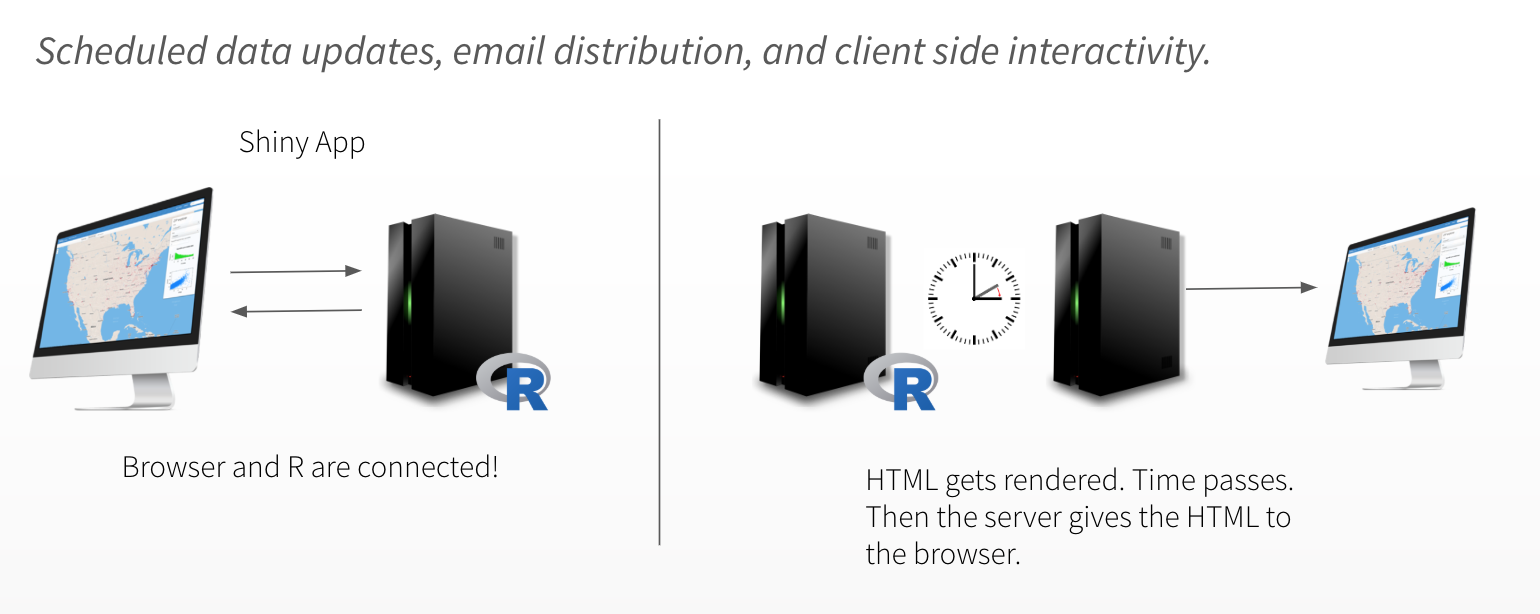
\includegraphics{imgs/shiny-alt/rmd-diagram.png}
\caption{Publishing R Markdown}
\end{figure}

\textbf{Publishing R Markdown to RStudio Connect}

\begin{itemize}
\tightlist
\item
  \textbf{Publishing Destination}
\end{itemize}

When publishing documents to RStudio Connect, you may encounter other
deployment options depending on your content.

\begin{itemize}
\item
  RPubs documents are (1) always public, (2) always self-contained, and
  (3) and cannot contain any Shiny content.
\item
  Choose ``RStudio Connect'' to publish to your RStudio Connect server.
\item
  \textbf{Publish Source Code}
\end{itemize}

Publishing the document with source code means that your R Markdown file
(.Rmd) will be deployed to RStudio Connect. This file is rendered
(usually to HTML) on the server.

Publishing only the finished document means that the HTML file you
rendered locally is deployed to RStudio Connect.

We recommend publishing your documents with source code, as it allows
you to re-render the document with RStudio Connect (on a weekly
schedule, for example). If the document cannot be rendered by RStudio
Connect because of files or data sources that are unavailable on the
server, choose ``Publish finished document only'' so others can view
your work.

\begin{itemize}
\tightlist
\item
  \textbf{Document Selection}
\end{itemize}

It is possible to link together multiple R Markdown documents to make a
multi-page document, so this is your chance to indicate that you've done
this, and to publish all the documents at once. In most cases however
you'll want to publish just the current document.

\begin{itemize}
\item
  \href{https://docs.rstudio.com/connect/user/publishing.html\#publishing-documents}{RStudio
  Connect Publishing Guide}
\item
  \href{https://rmarkdown.rstudio.com/}{R Markdown}
\end{itemize}

\begin{figure}
\centering
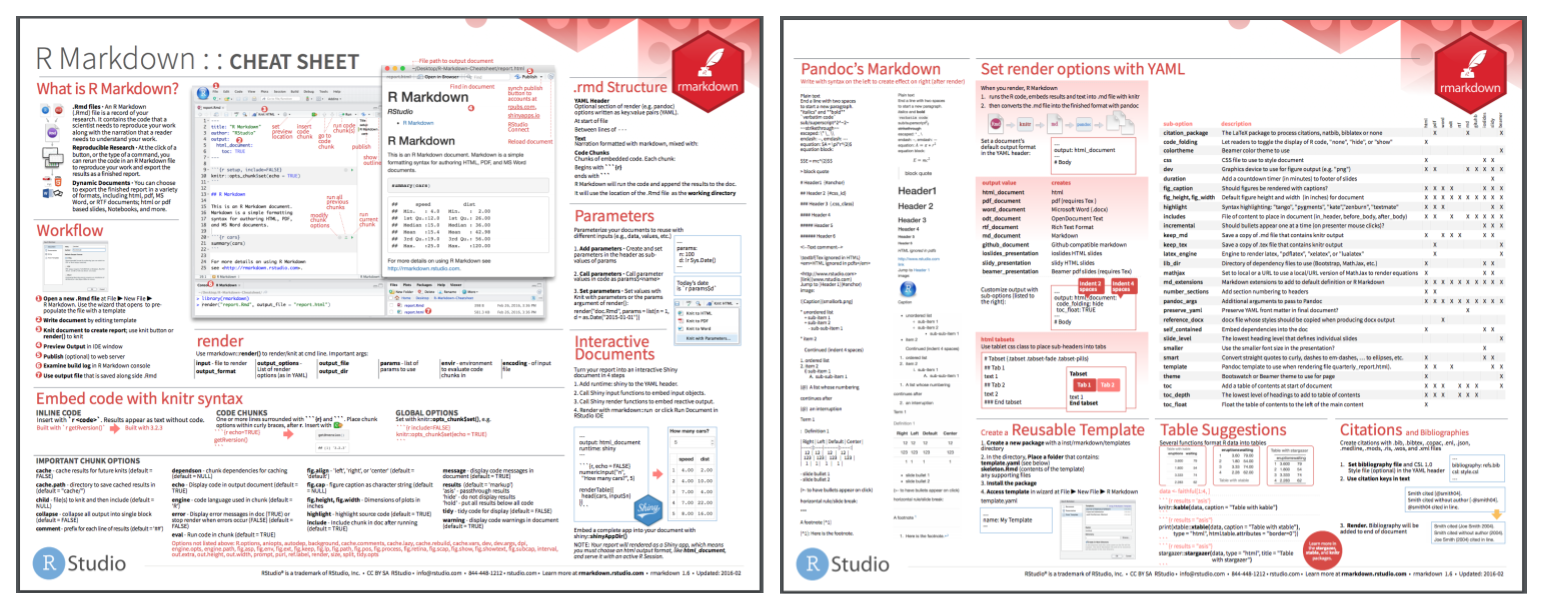
\includegraphics{imgs/shiny-alt/rmd-cheatsheet.png}
\caption{R Markdown Cheatsheet Preview}
\end{figure}

\hypertarget{references-and-resources-3}{%
\subsubsection{References and
Resources}\label{references-and-resources-3}}

\begin{itemize}
\tightlist
\item
  \href{https://docs.rstudio.com/connect/user/r-markdown.html}{R
  Markdown in the RStudio Connect User Guide}
\item
  \href{https://rmarkdown.rstudio.com/articles.html}{R Markdown
  Reference Articles}
\item
  \href{https://rviews.rstudio.com/2018/11/01/r-markdown-a-better-approach/}{RViews
  Blog: Communicating results with R Markdown by Nathan Stephens}
\item
  \href{https://rviews.rstudio.com/2018/05/16/replacing-excel-reports-with-r-markdown-and-shiny/}{RViews
  Blog: Enterprise Dashboards with R Markdown by Nathan Stephens}
\end{itemize}

\hypertarget{workshop-exercise-r-markdown}{%
\subsection{Workshop Exercise: R
Markdown}\label{workshop-exercise-r-markdown}}

\textbf{First: Create your own R markdown document (New File)}

\textbf{Discussion:}

\emph{Consider R Markdown}

\begin{itemize}
\tightlist
\item
  How does an R Markdown document scale?
\item
  What types of interactivity can be added to R Markdown?
\end{itemize}

\textbf{Deliverable:}

\begin{itemize}
\tightlist
\item
  Create a decision matrix comparing Shiny to R Markdown
\end{itemize}

\begin{figure}
\centering
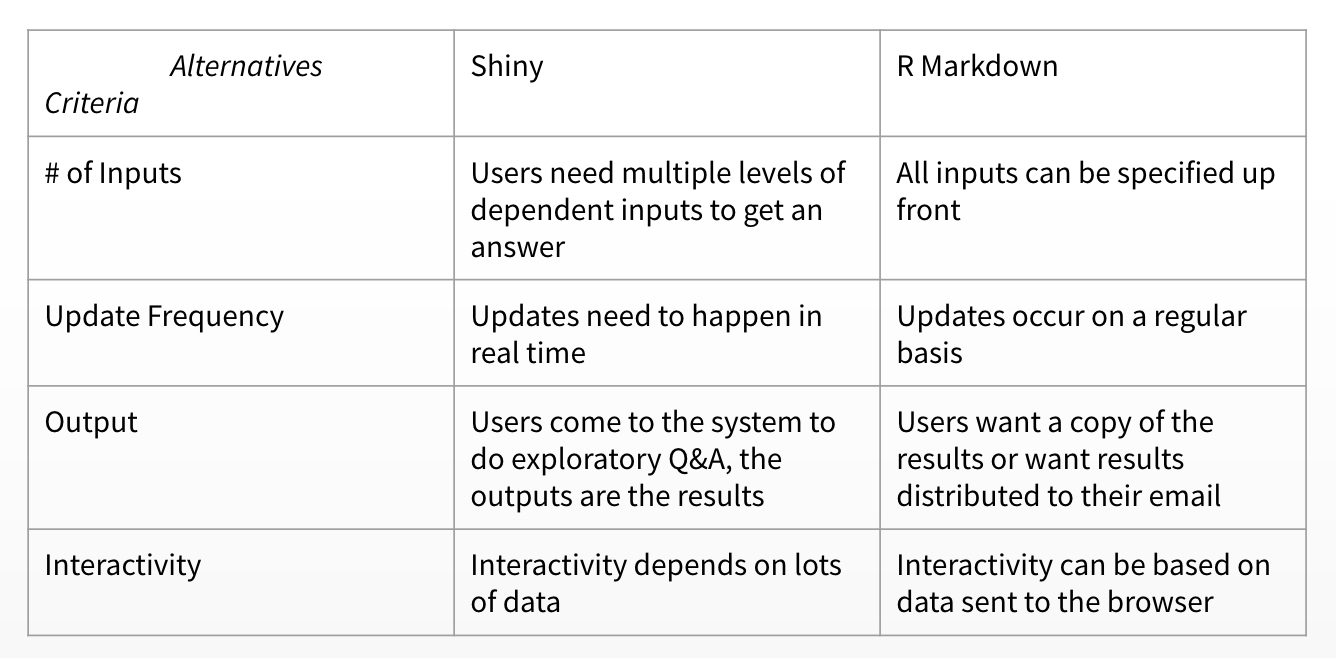
\includegraphics{imgs/shiny-alt/rmd-answers.png}
\caption{Rmd Exercise}
\end{figure}

\hypertarget{shiny-async}{%
\chapter{Shiny Async}\label{shiny-async}}

\hypertarget{references-and-resouces}{%
\subsubsection{References and Resouces}\label{references-and-resouces}}

\begin{itemize}
\tightlist
\item
  \href{https://resources.rstudio.com/webinars/scaling-shiny-apps-with-async-programming-june-2018}{Webinar
  - Scaling Shiny apps with asynchronous programming}
\item
  \href{https://github.com/rstudio/webinars/blob/master/56-scaling-shiny-apps/Scaling\%20Shiny\%20apps\%20with\%20async\%20programming.pdf}{Webinar
  Slides}
\item
  \href{http://shiny.rstudio.com/articles/async.html}{Shiny Dev Center
  Article: Improving scalability with async programming}
\end{itemize}


\end{document}
